\documentclass[12pt,a4paper,twoside]{article}
\usepackage{labor}
\begin{document}

%fill for cover and header creation
\newcommand\laboratorynumber{2}
\title{Oszillograph}
\newcommand\supervisor{Ditlbacher, Harald}
\newcommand\groupnumber{42}

\newcommand\participantonelastname{Eisner}
\newcommand\participantonefirstname{Nico}
\newcommand\participantoneid{12214121}
\newcommand\participanttwolastname{Waldl}
\newcommand\participanttwofirstname{Philip}
\newcommand\participanttwoid{12214120}
\author{\participantonelastname \ \& \participanttwolastname}

\newcommand\degreeid{UB 033 678}
\newcommand\semester{23WS}
\date{20.10.2023}

%select correct course title
%\newcommand\coursetitle{Einführung in die \\ physikalischen Messmethoden}
%\newcommand\coursetitle{Laborübungen 1: \\ Mechanik und Wärme}
\newcommand\coursetitle{Laborübungen 2: \\ Elektrizität, Magnetismus, Optik}
%\newcommand\coursetitle{Fortgeschrittenen Praktikum 1: \\ Technische Physik}
%\newcommand\coursetitle{Fortgeschrittenen Praktikum 2: \\ Allgemeine Physik}

%\begin{titlepage}
   \begin{center}
       \begin{figure}[H]
            \begin{minipage}[h]{30mm}
                \centerline{
\includegraphics[height=15mm]{cover_nudes/tugraz.png}}
            \end{minipage}
            \hfill
            \begin{minipage}[h]{30mm}
                \centerline{
\includegraphics[height=15mm]{cover_nudes/nawi_graz.png}}
            \end{minipage}
            \hfill
            \begin{minipage}[h]{30mm}
                \centerline{
\includegraphics[height=15mm]{cover_nudes/uni-graz.png}}
            \end{minipage}
        \end{figure}
        
        \large{\emph{Institut für Experimentalphysik der Technischen Universität Graz \\
        \& Institut für Physik der Universität Graz}} \\
        \vspace{5mm}
        
        {\Huge \textbf{\coursetitle}}
        \vspace{5mm}
        
        {\huge \laboratorynumber: \thetitle}
    \end{center}
    
    \vfill
    
    \begin{table}[H]
        \LARGE
        \centering
        \begin{tabular}{r l}
            Betreuer:       & \supervisor \\
            Gruppennummer:  & \groupnumber \\
            \\
            Name:           & \participantonelastname, \participantonefirstname \\
            Matrikelnummer: & \participantoneid \\
            Name:           & \participanttwolastname, \participanttwofirstname \\
            Matrikelnummer: & \participanttwoid \\
            \\
            Kennzahl:       & \degreeid \\
            Datum:          & \semester \ | \thedate
        \end{tabular}
    \end{table}
    \vspace{4cm}
\end{titlepage}
\clearpage
\setcounter{page}{1}

%\maketitle %short title alternative

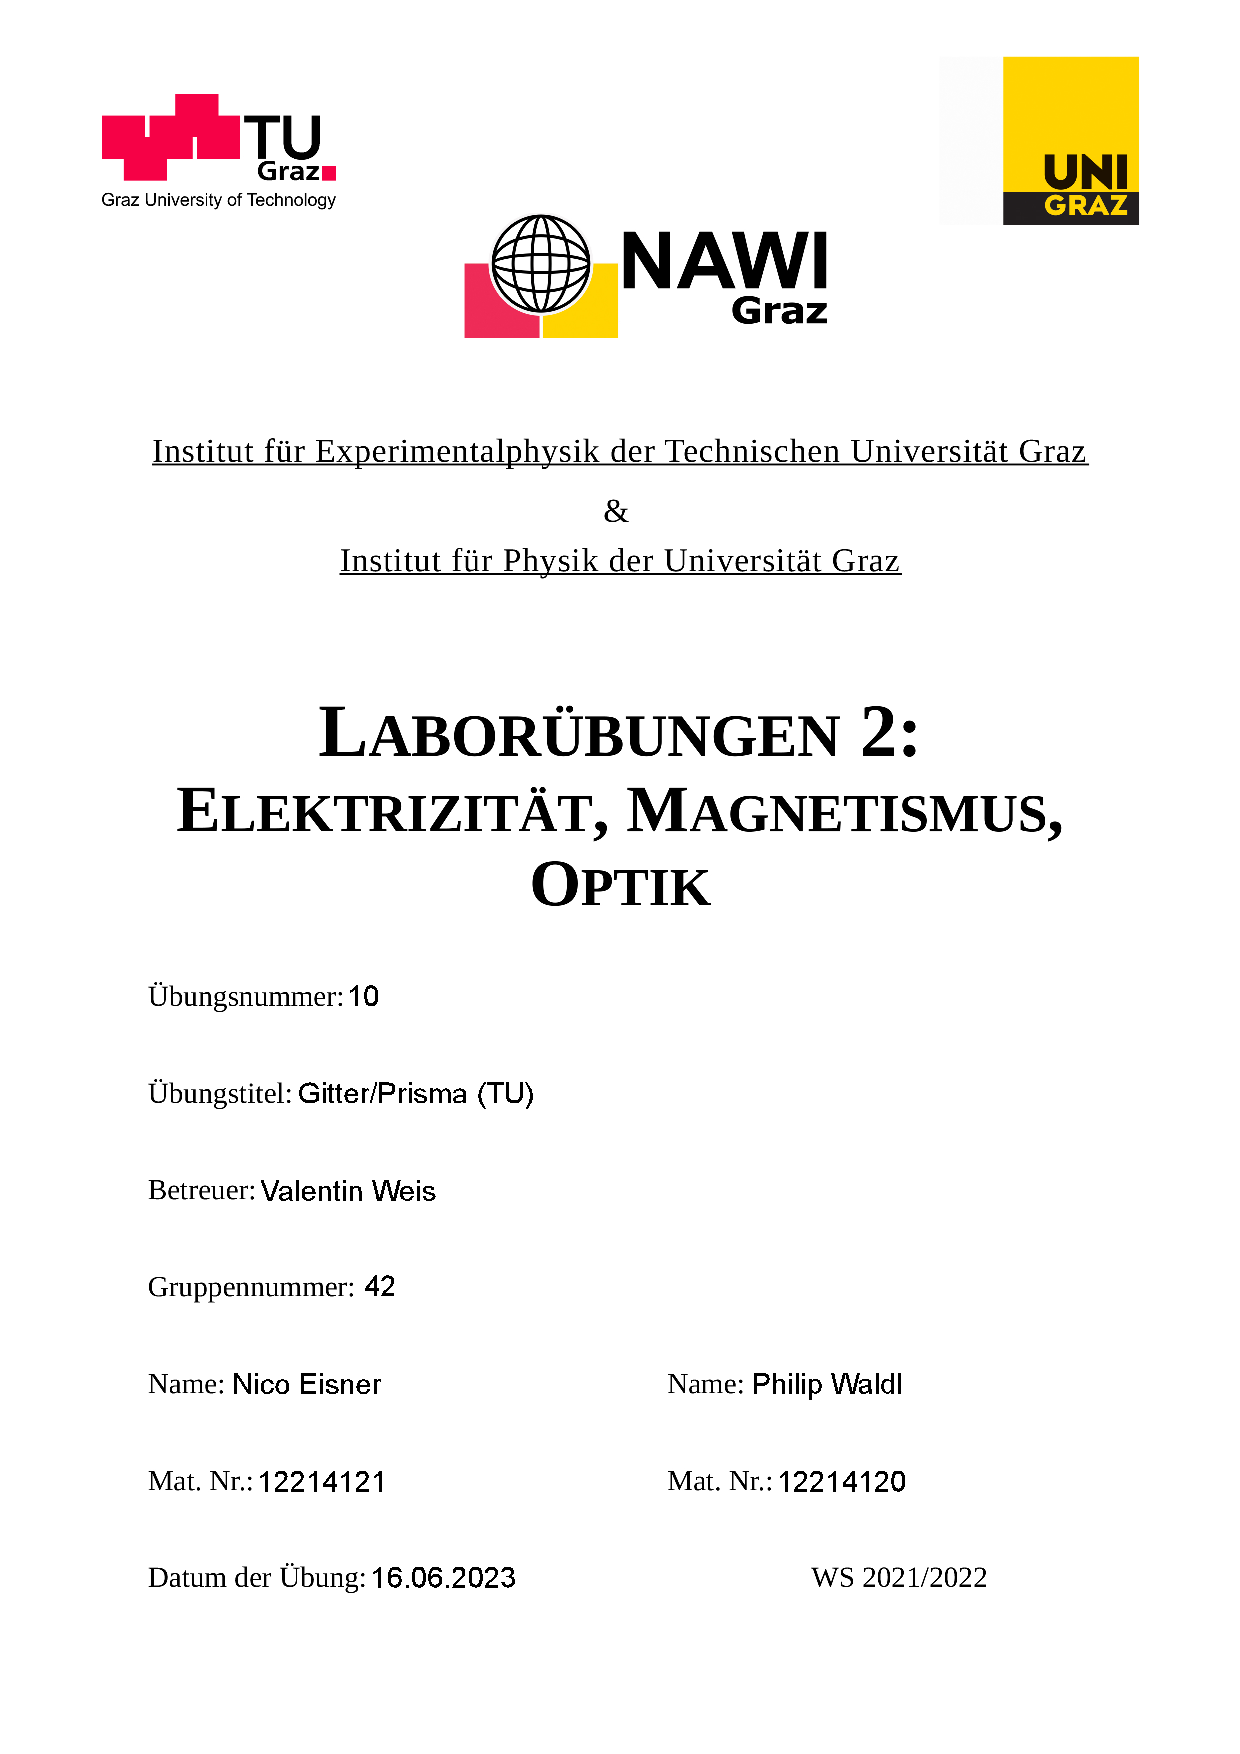
\includepdf[pages={1}]{../Deckblätter/Deckblatt_Gitter.pdf}

\tableofcontents
\newpage

\section{Aufgabenstellung} %jo beschreibn wos gmocht host ------------------------------

Der Versuch Oszillograph geht, wie der Name bereits vermuten lässt, auf die Funktion des Oszilloskopes ein, was in erster Linie die grafische Darstellung elektrischer Spannungen über einen bestimmten Zeitraum beinhaltet.
Mit drei verschiedenen elektrischen Schaltungen soll dies ausprobiert und in diesem Protokoll veranschaulicht werden. 
Die tatächliche Aufgabenstellung sieht hierfür wie folgt aus:

\begin{itemize}
    \item Serienschaltung (Trafo, Kondensator, Widerstand)
    \begin{itemize}
        \item Ermittlung des Phasenversatzes $\phi$
        \item Ermittlung von der Zerfallskonstante $\tau$
    \end{itemize}
    \item Serienschwingkreis (Trafo, Kondensator, Widerstand, Potentiometer)
    \begin{itemize}
        \item Zeichnen der von Kriechfall, Schwingfall, Aperiodischer Grenzfall des Serienschwingkreises
        \item Induktion der Spulte mit und ohne Eisenkern $L_{mitEisenkern}$ / $L_{ohneEisenkern}$
    \end{itemize}
    \item Frequenzbestimmung (Piezo)
    \begin{itemize}
        \item Eigenfrequenz des Stuhles $f_{Stuhl}$
        \item Eigenfrequenz des Piezos $f_{Piezo}$
    \end{itemize}
\end{itemize}

\noindent
Alle Informationen und Methodiken wurden uns von der Technischen Universität bereitgestellt \cite{teachcenter1}. 



\section{Voraussetzungen \& Grundlagen} %Grundlagen erklären, Formeln mit erklärung

Wie bereits in der Aufgabenstellung erwähnt werden Oszilloskope hauptsächlich zur grafischen Darstellung elektrischer Spannungen eingesetzt.  
Das Hauptbestandsteil des Gerätes ist eine Braun'sche Röhre und sieht im groben Aufbau wie folgt aus:

\begin{figure}[H]
    \centering
    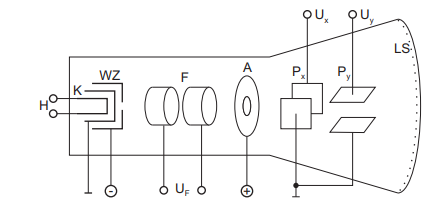
\includegraphics[width=0.5\linewidth]{nudes/OszilloskopAufbau.png}
    \caption{Grundlegender Aufbau eines Oszilloskop/Braun'sche Röhre \cite{teachcenter1}}
    \label{fig:Aufbau Oszilloskop}
\end{figure}

\noindent
Die beheizte Kathode K beschleunigt Elektronen gegen eine Anode A. Diese besitzt eine Öffnung, durch die die Elektronen hindurchfliegen und mit Hilfe der Ablenkplatten $P_{x}$ (horizontal) und $P_{y}$ (vertikal) an die richtige Position des Leuchtschirms LS gelenkt werden. 
Ein Oszilloskop besitzt außerdem einen Triggerungsmechanismus. Dieser sorgt dafür, dass das Signal beim erreichen des Bildschirmendes kurz pausiert wird, damit dieses wieder zum Anfang springen kann. \newline

\noindent
Zur erfolgreichen Durchführung des Versuches ist auch der Schwingkreis von Bedeutung. Dies ist im Prinzip eine einfache Schaltung, bestehend aus Kapazität, Induktivität und Widerstand.
Mittels Gleichung

    \begin{equation}
        \label{eq:SchwingkreisGleichungFälle}
        \centerline{$\lambda^2 + \lambda \frac{R}{L} + \frac{1}{LC} = 0 $}
    \end{equation}

\noindent
können hier drei verschiedene Fälle unterschieden werden:

\begin{itemize}
    \item $R^2C - 4L$ > 0: Kriechfall
    \item $R^2C - 4L$ = 0: Aperiodischer Grenzfall
    \item $R^2C - 4L$ < 0: Schwingfall
\end{itemize}

\noindent
Für die Auswertung des Versuches ist auch die Formel für die Phasenverschiebung $\Phi$ wichtig, welche aus dem gemessenen Zeitunterschied und der Frequenz berechnet werden kann.

\begin{equation}
    \label{eq:Phasenversatz}
    \centerline{$\Phi = \frac{360°}{T}*\Delta t = 360° * \Delta t * f$}
\end{equation}

\noindent
Außerdem wird für den Vergleich der gemessenen Zerfallskonstante mit der berechneten noch eine Formel für letztere benötigt.

\begin{equation}
    \label{eq:Zerfallskonstante}
    \centerline{$\tau = R*C$}
\end{equation}


\section{Versuchsanordnung} %mit skizze kurz beschreiben ------------------------------

Als Grundstein des gesamten Experimentes steht natürlich das Oszilloskop, abgebildet in nachstehender Grafik.

\begin{figure}[H]
    \centering
    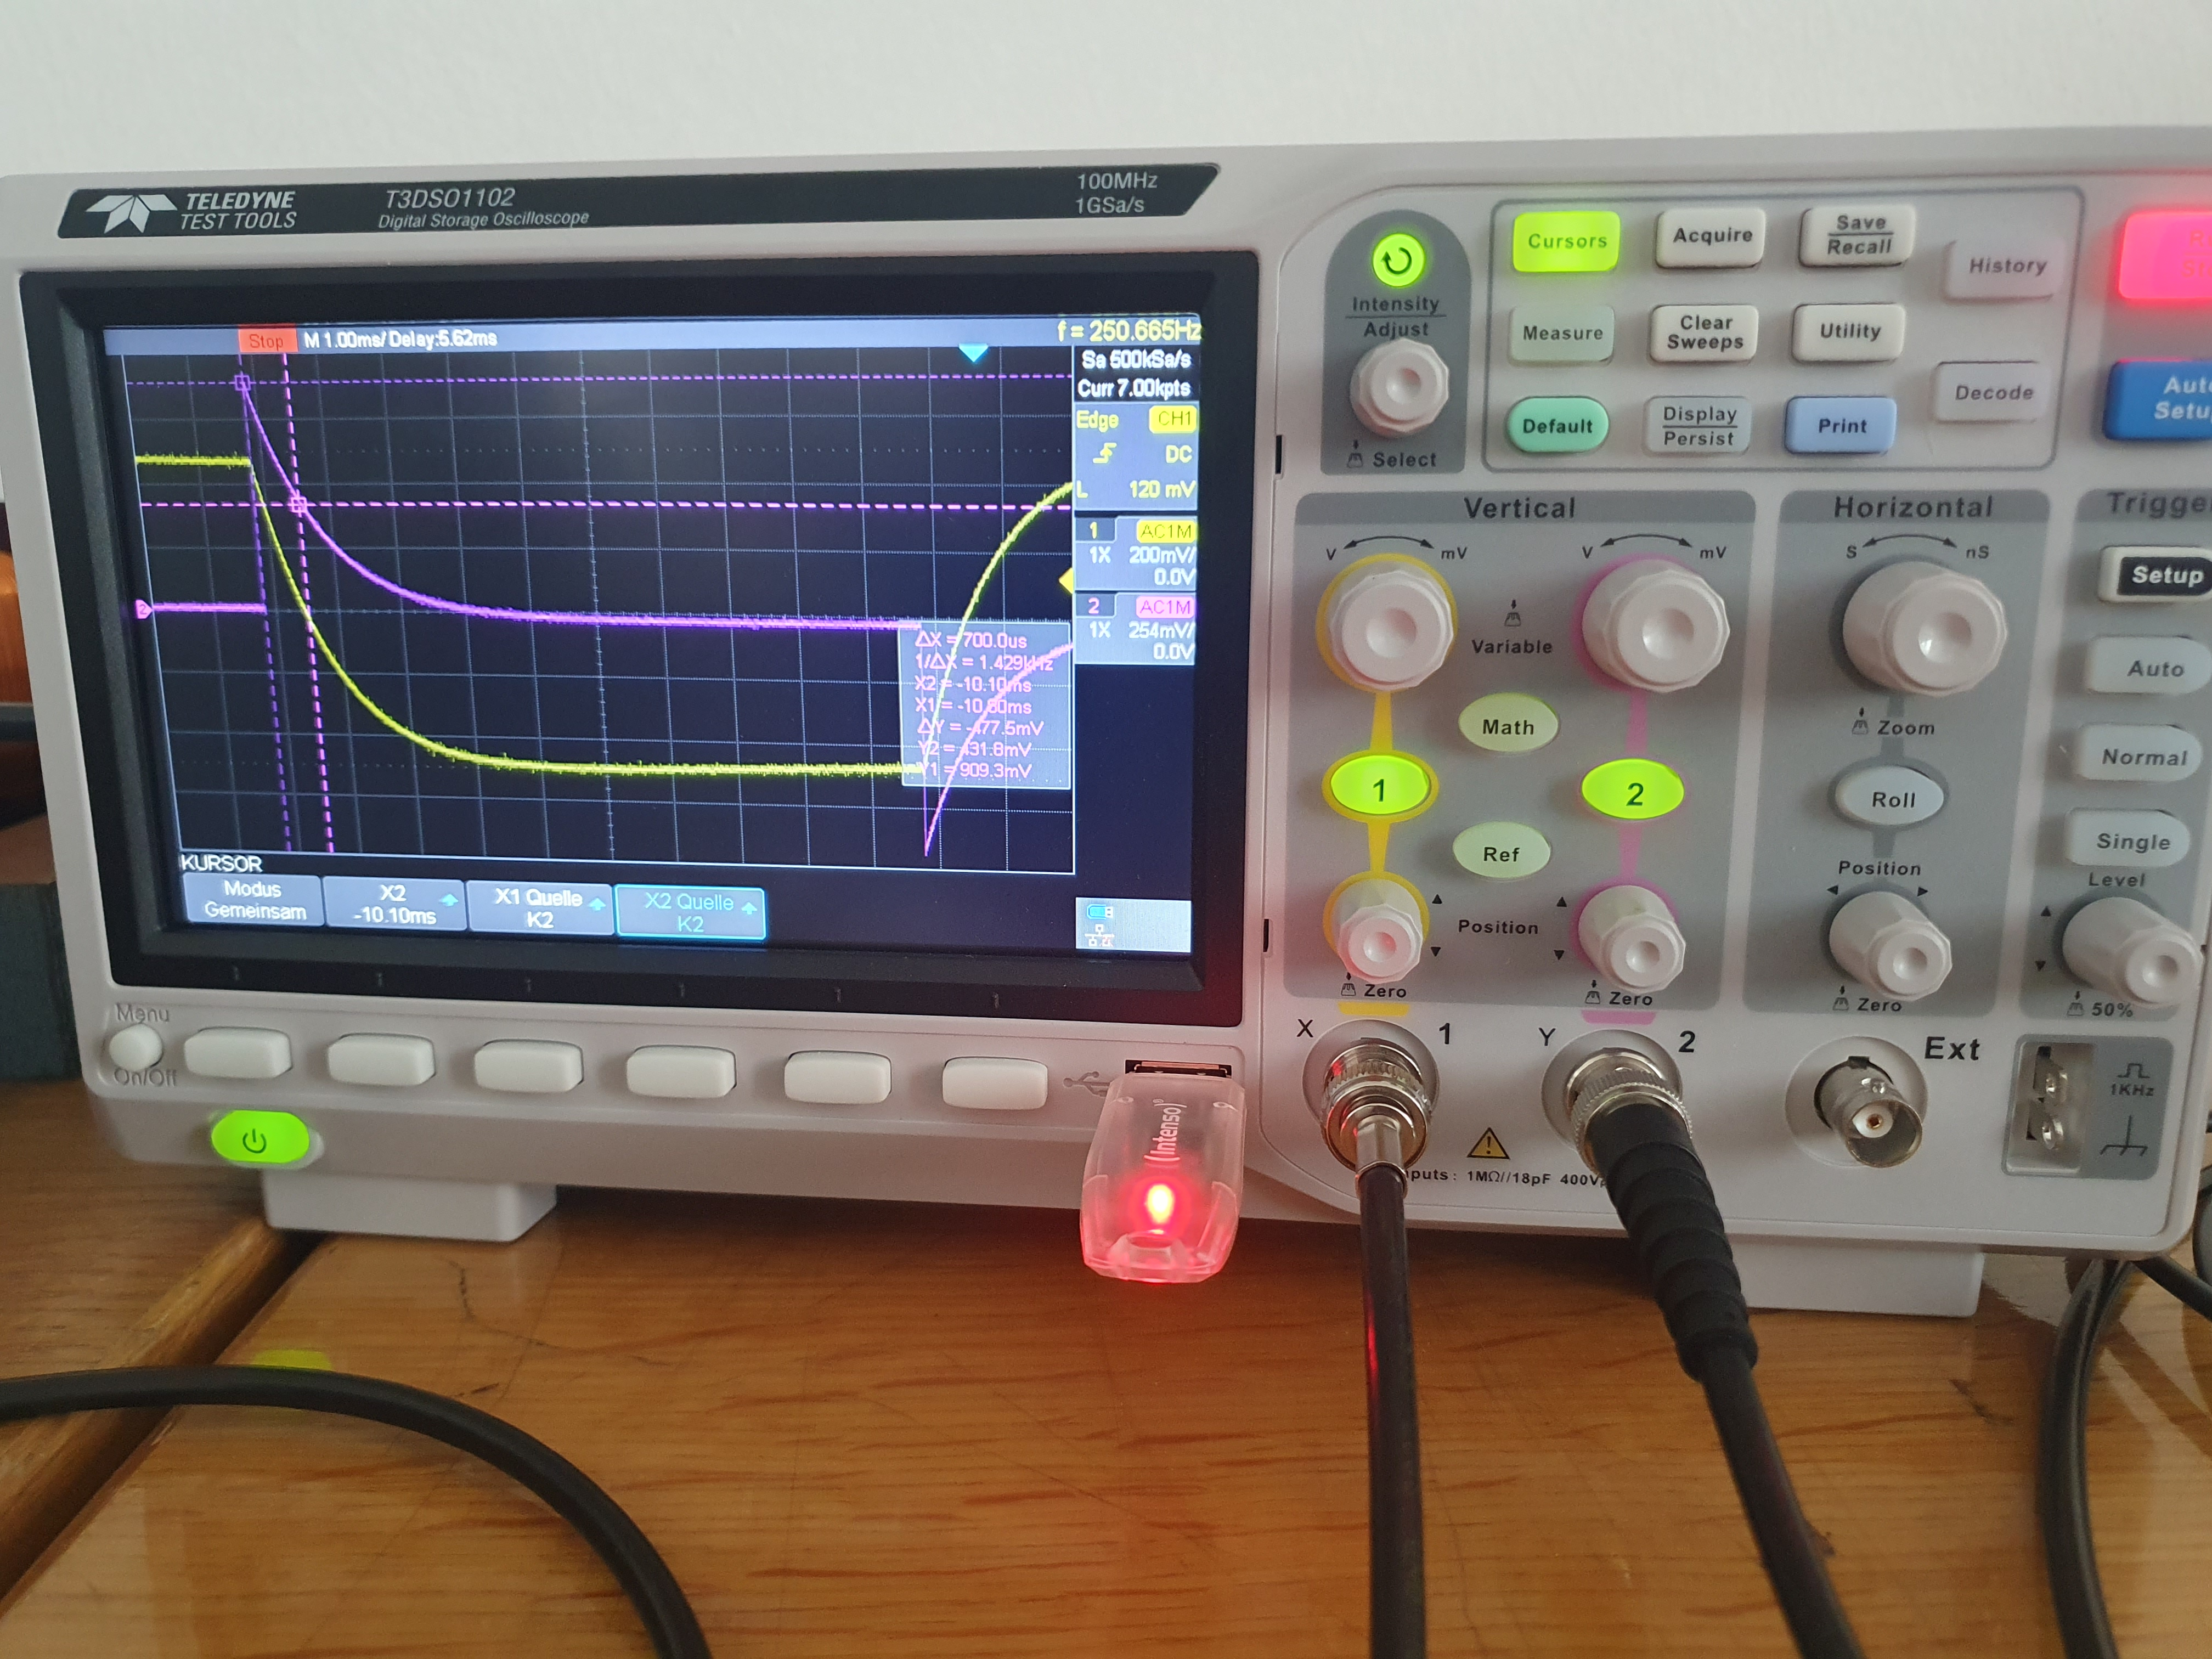
\includegraphics[width=0.6\linewidth, angle=0]{nudes/Osziloskop.jpg}
    \caption{Oszilloskop}
    \label{fig:Oszilloskop}
\end{figure}

\noindent
Auch Trafo und Frequenzgenerator, zu sehen in folgenden Abbildungen, sind weitere, wichtige Elemente des Versuches. 

\begin{figure}[H]
    \centering
    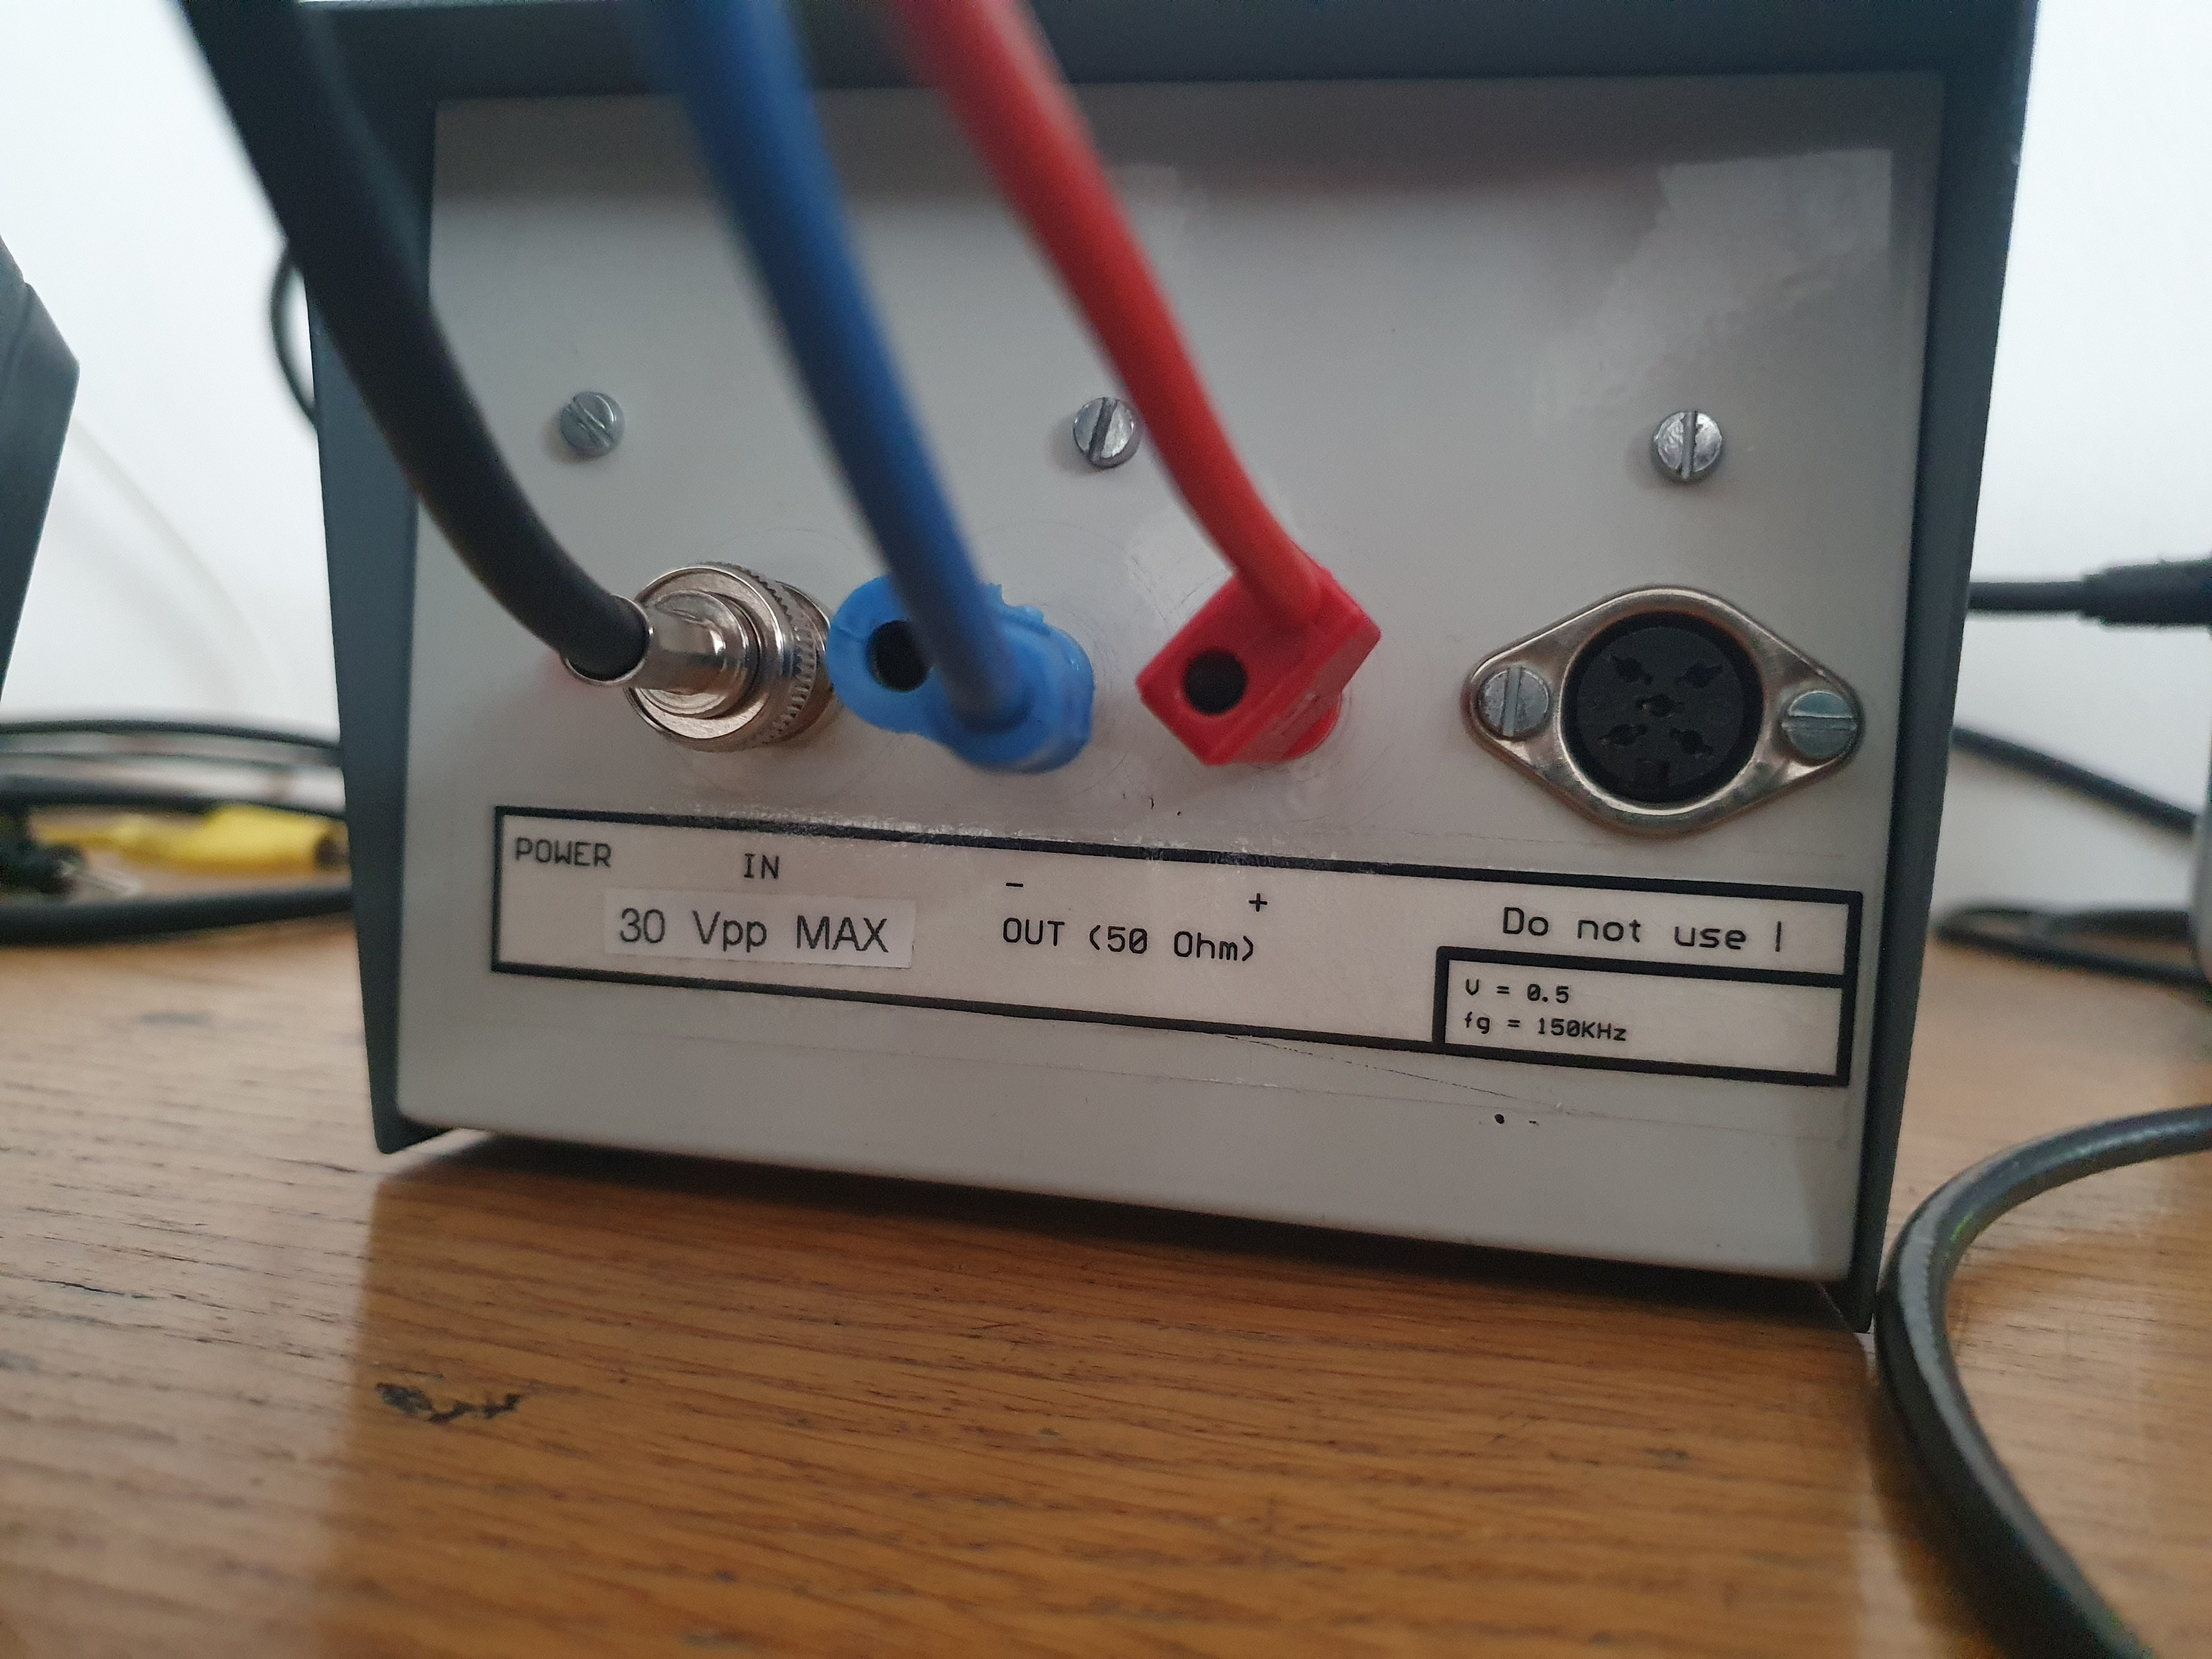
\includegraphics[width=0.6\linewidth, angle=0]{nudes/Trafo.jpg}
    \caption{Trafo}
    \label{fig:Trafo}
\end{figure}

\begin{figure}[H]
    \centering
    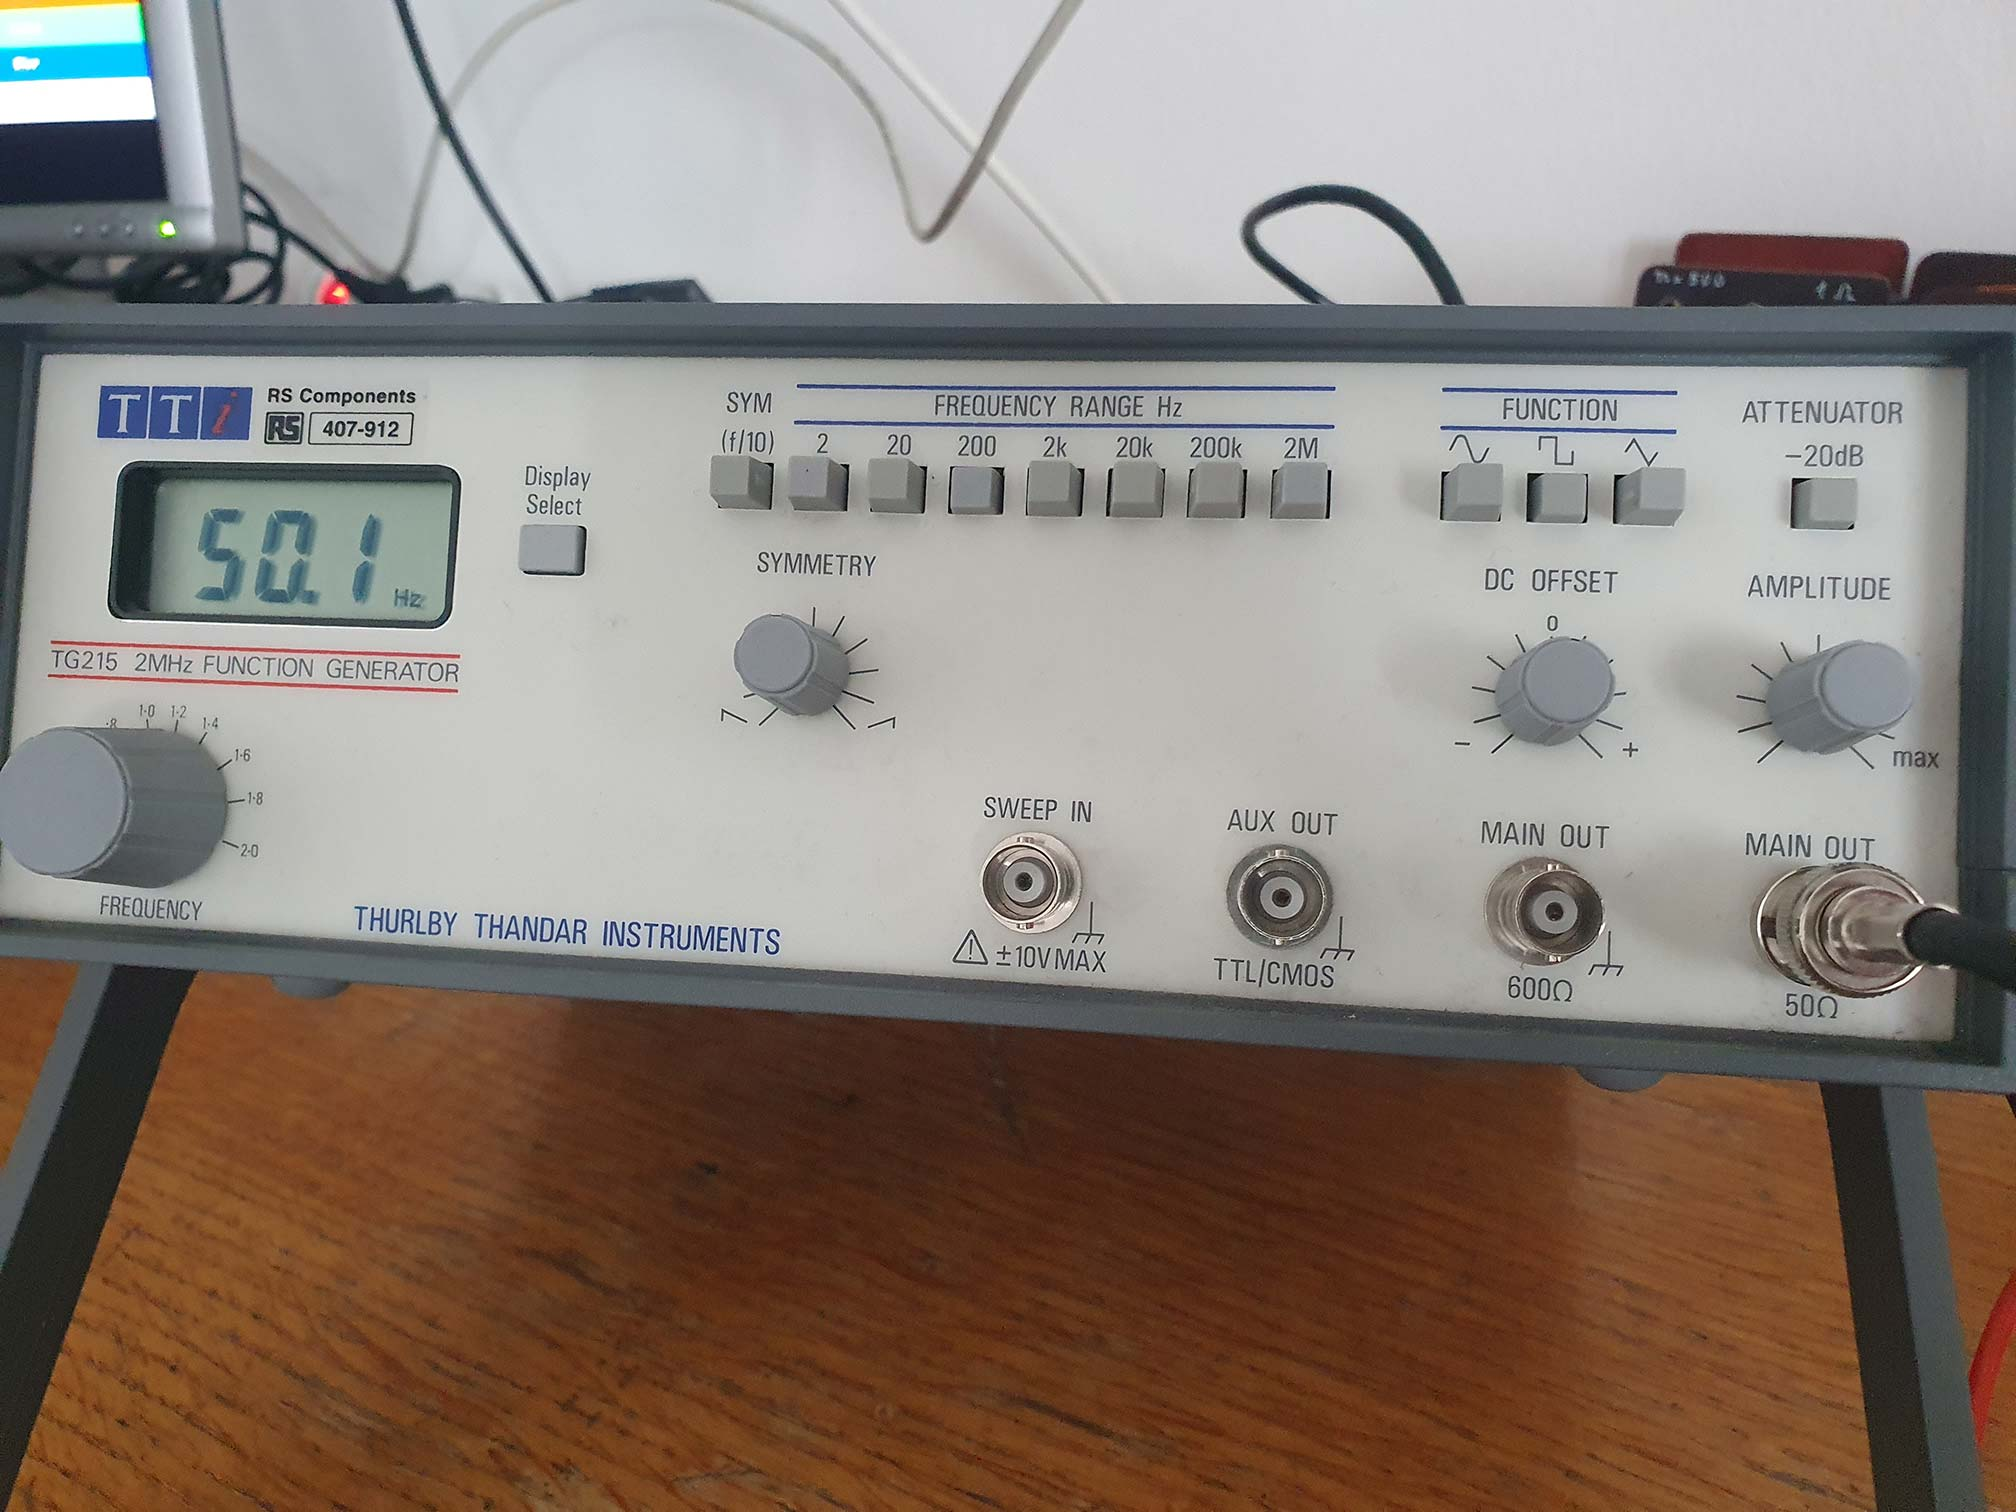
\includegraphics[width=0.6\linewidth, angle=0]{nudes/Frequenzgenerator.jpg}
    \caption{Frequenzgenerator}
    \label{fig:Frequenzgenerator}
\end{figure}

\noindent
Weiters kamen dann noch einige kleinere Utensilien zum Einsatz:

\begin{figure}[H]
    \centering
    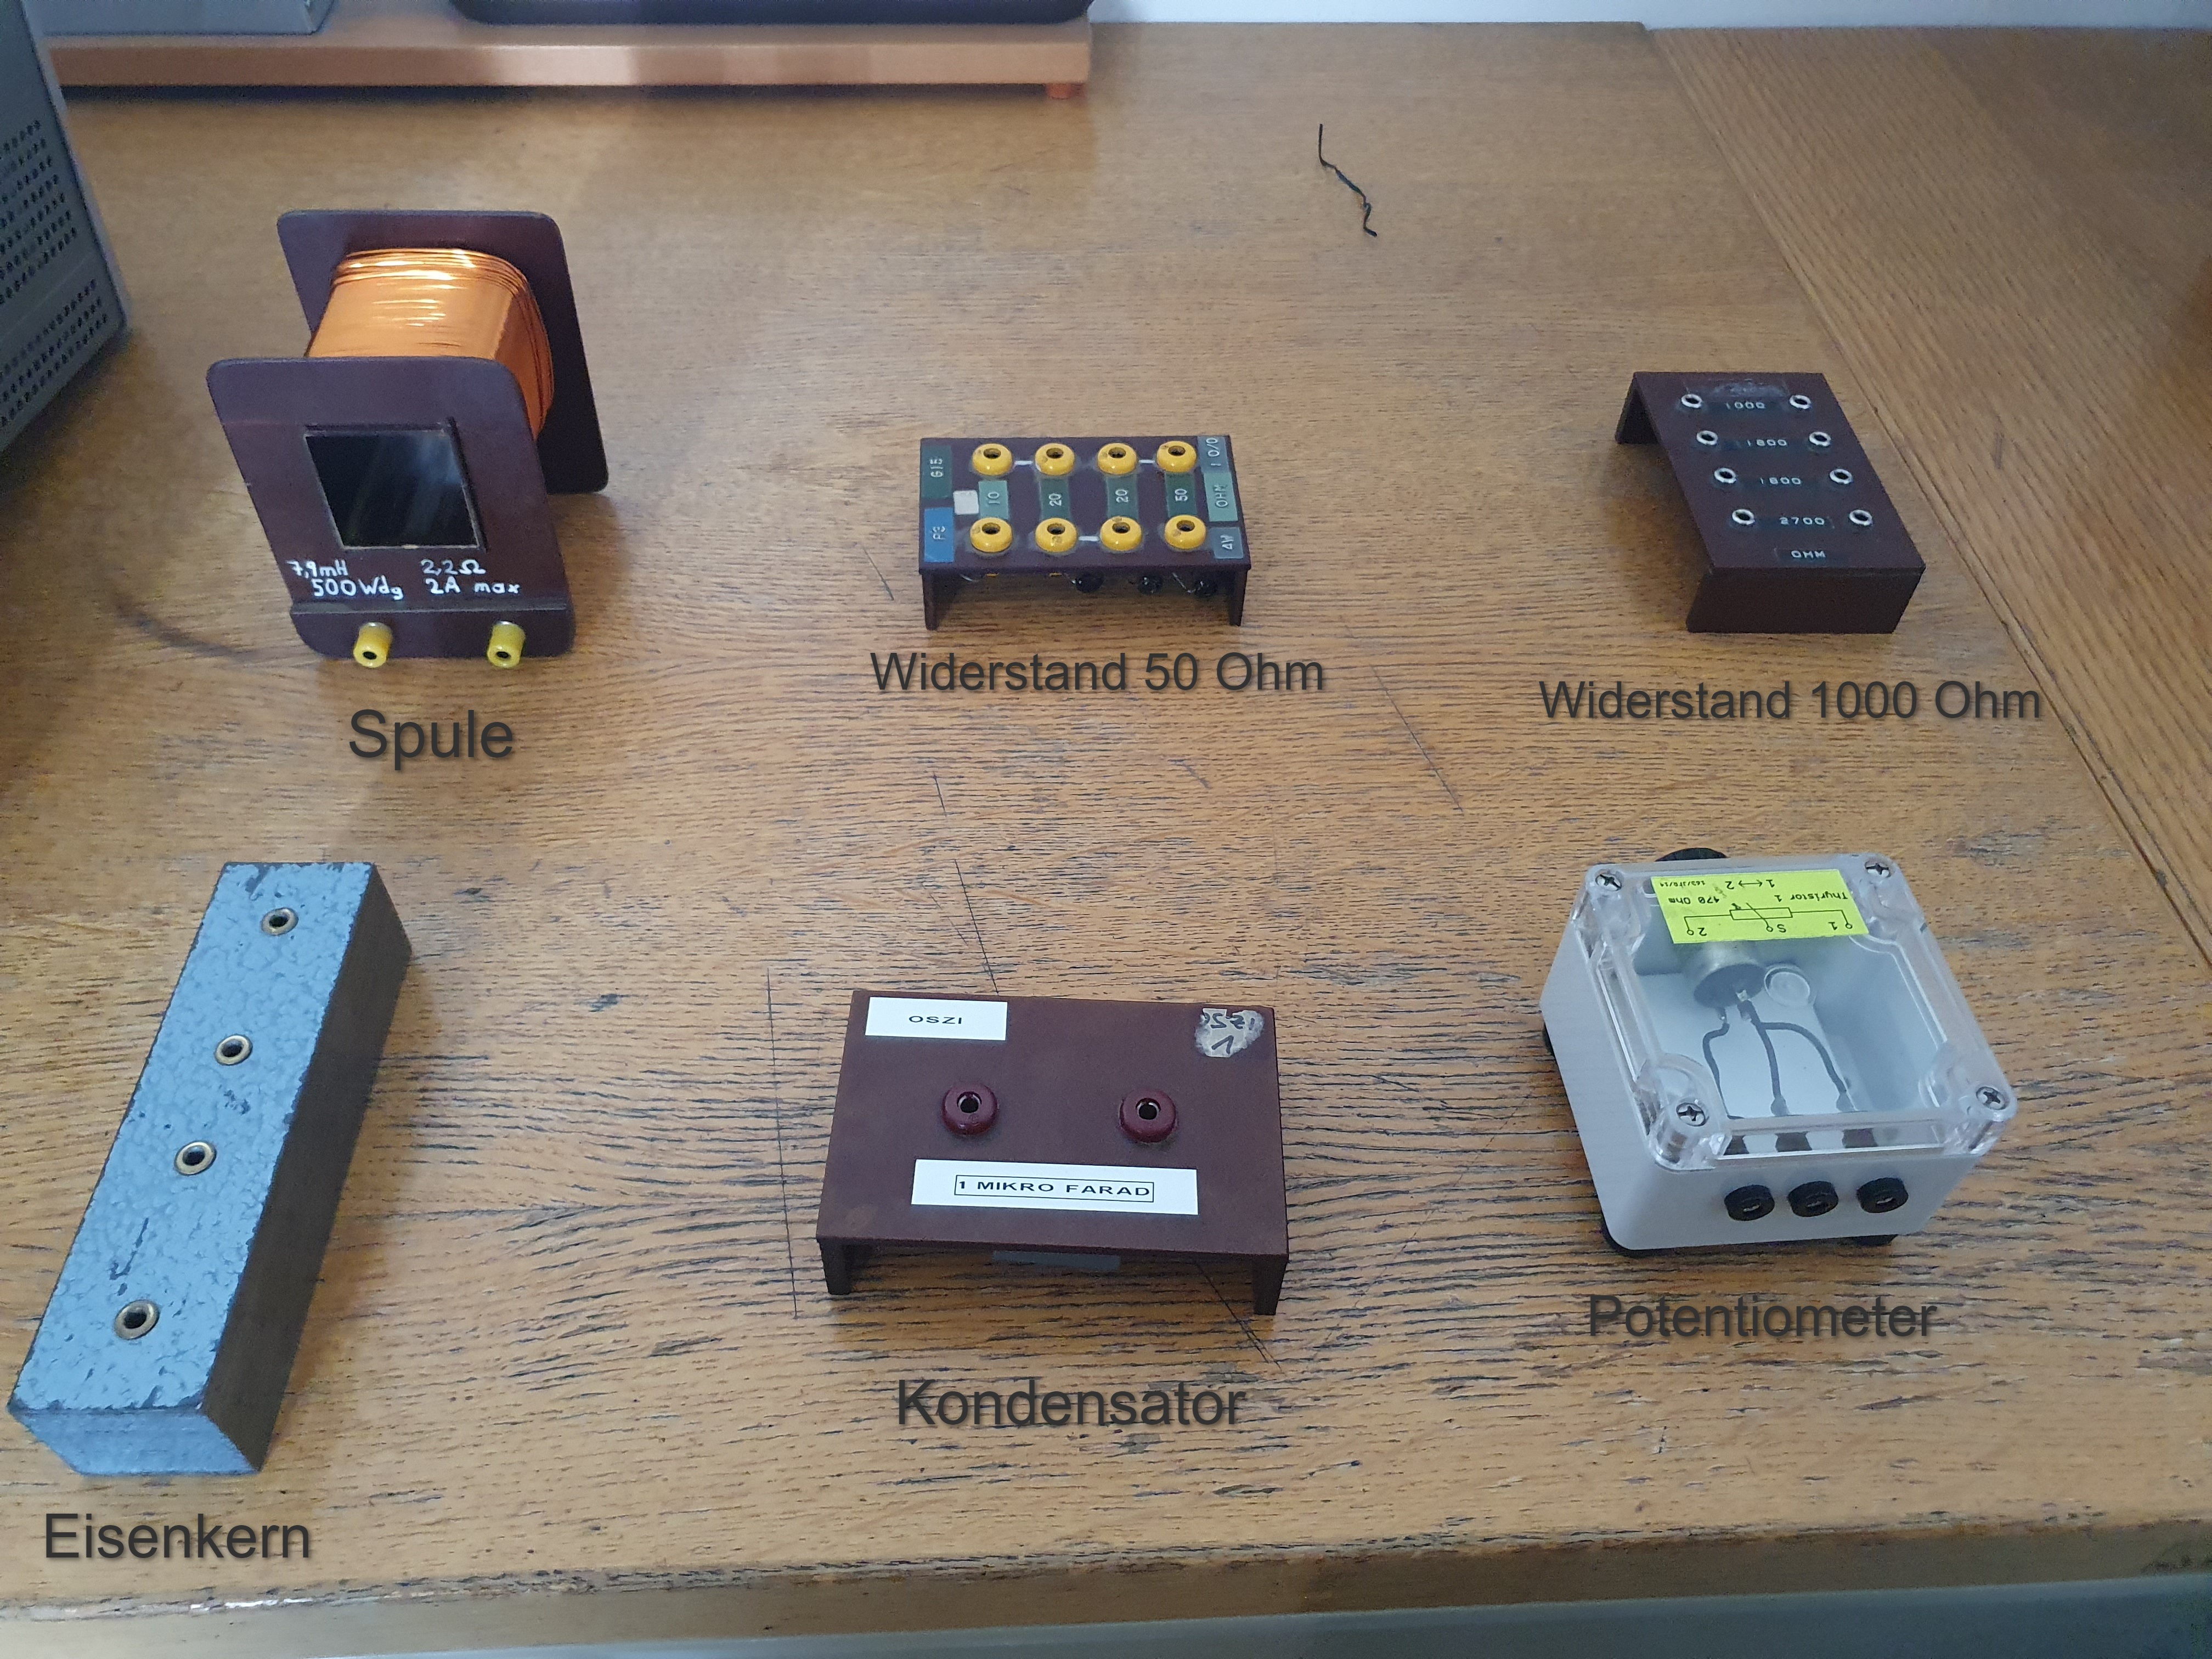
\includegraphics[width=0.6\linewidth, angle=0]{nudes/Utensilien.jpg}
    \caption{Utensilien}
    \label{fig:Utensilien}
\end{figure} 

\noindent
Basierend darauf war der Versuch dann in drei Teilversuche gegliedert. Im ersten Abschnitt davon sollte eine Serienschaltung, bestehend aus einem Widerstand R = 1000 Ohm, einem Kondensator C = 1 $\mu F$, einem Trafo und einem Frequenzgenerator aufgebaut- und dann an das Oszilloskop angeschlossen werden.
Der Schaltplan hierzu ist in folgender Abbildung zu erkennen:

\begin{figure}[H]
    \centering
    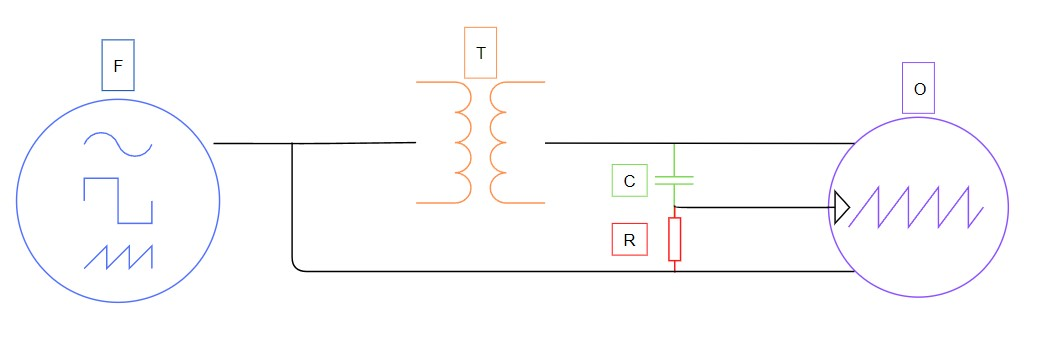
\includegraphics[width=0.6\linewidth, angle=0]{nudes/Serienschaltung gezeichnet.jpg}
    \caption{Schaltplan Serienschaltung}
    \label{fig:Schaltplan Serienschaltung}
\end{figure}

\noindent
Praktisch aufgebaut sieht der Versuch wie folgt aus:

\begin{figure}[H]
    \centering
    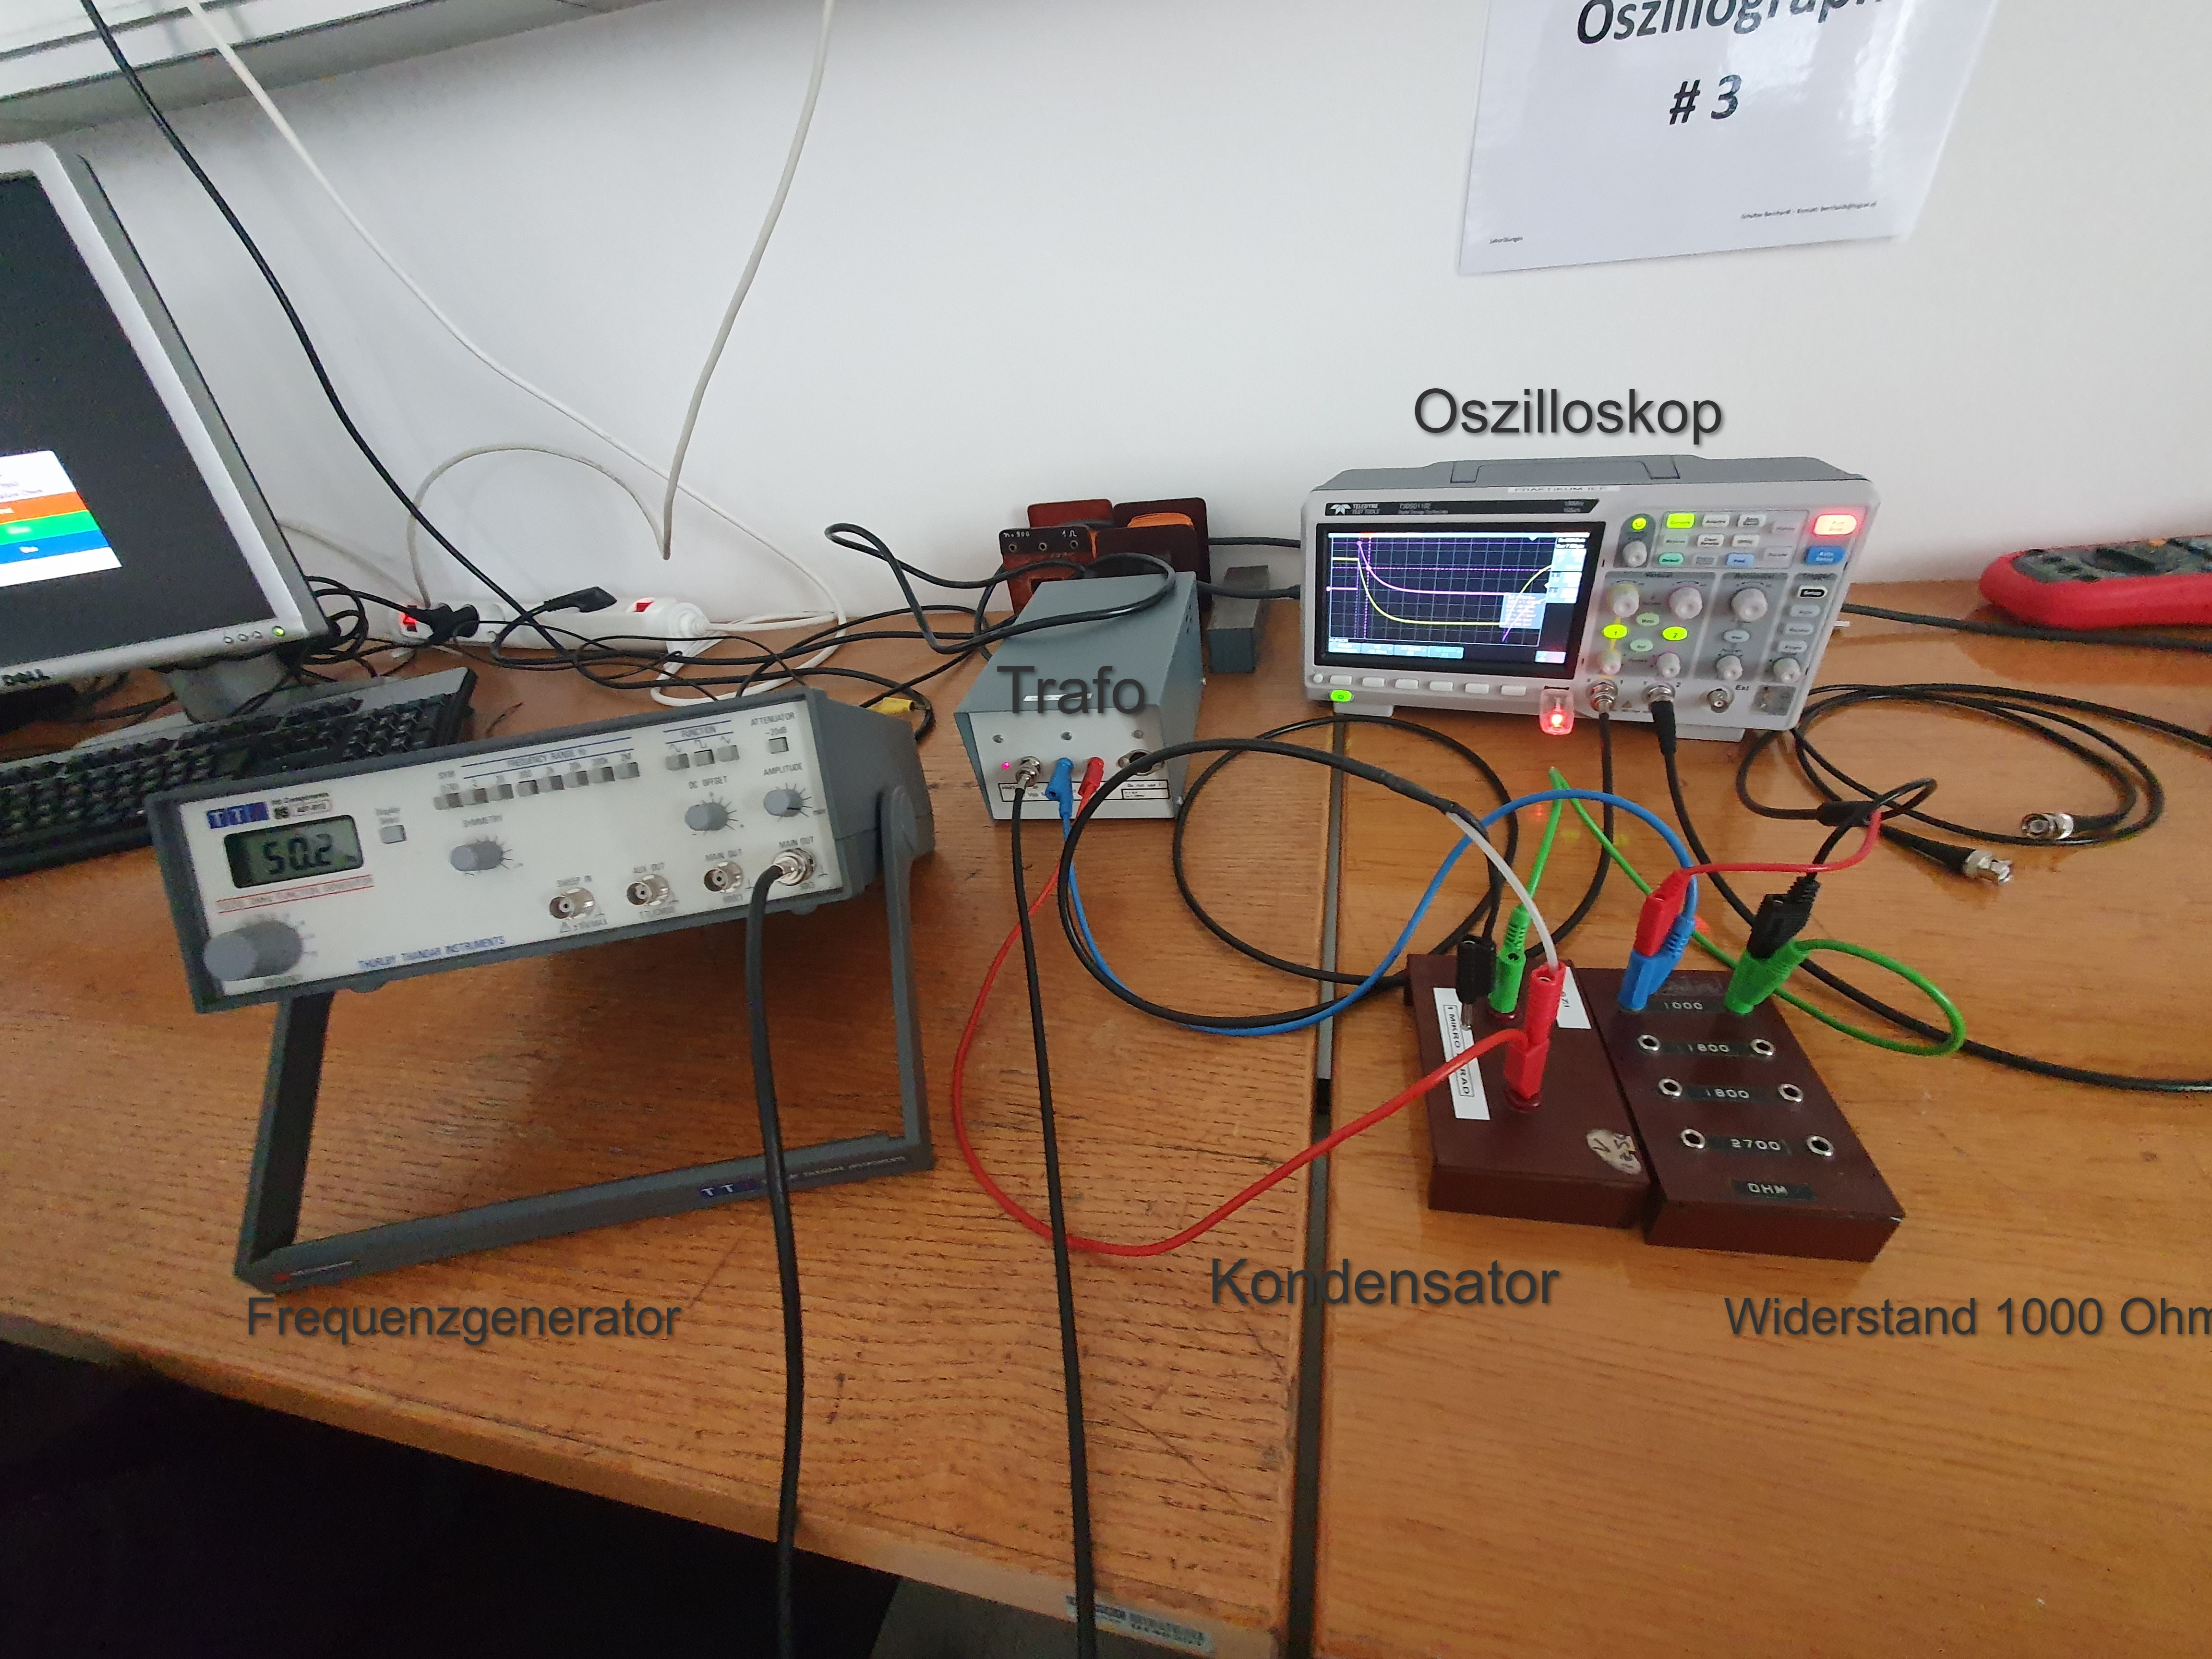
\includegraphics[width=0.6\linewidth, angle=0]{nudes/Aufbau Serienschaltung.jpg}
    \caption{Aufbau Serienschaltung}
    \label{fig:Aufbau Serienschaltung}
\end{figure} 

\noindent
Der Aufbau des zweiten Teiles kann sich mit der Grafik zum Schaltplan des Serienschwingkreises vorgestellt werden:

\begin{figure}[H]
    \centering
    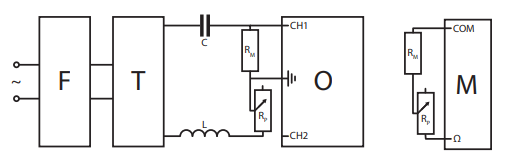
\includegraphics[width=0.6\linewidth, angle=0]{nudes/3.3 Serienschwingkreis.png}
    \caption{Schaltplan Serienschwingkreis}
    \label{fig:Schaltplan Serienschwingkreis}
\end{figure}

\noindent
In der Realität sieht die aufgebaute Schaltung dann so aus:

\begin{figure}[H]
    \centering
    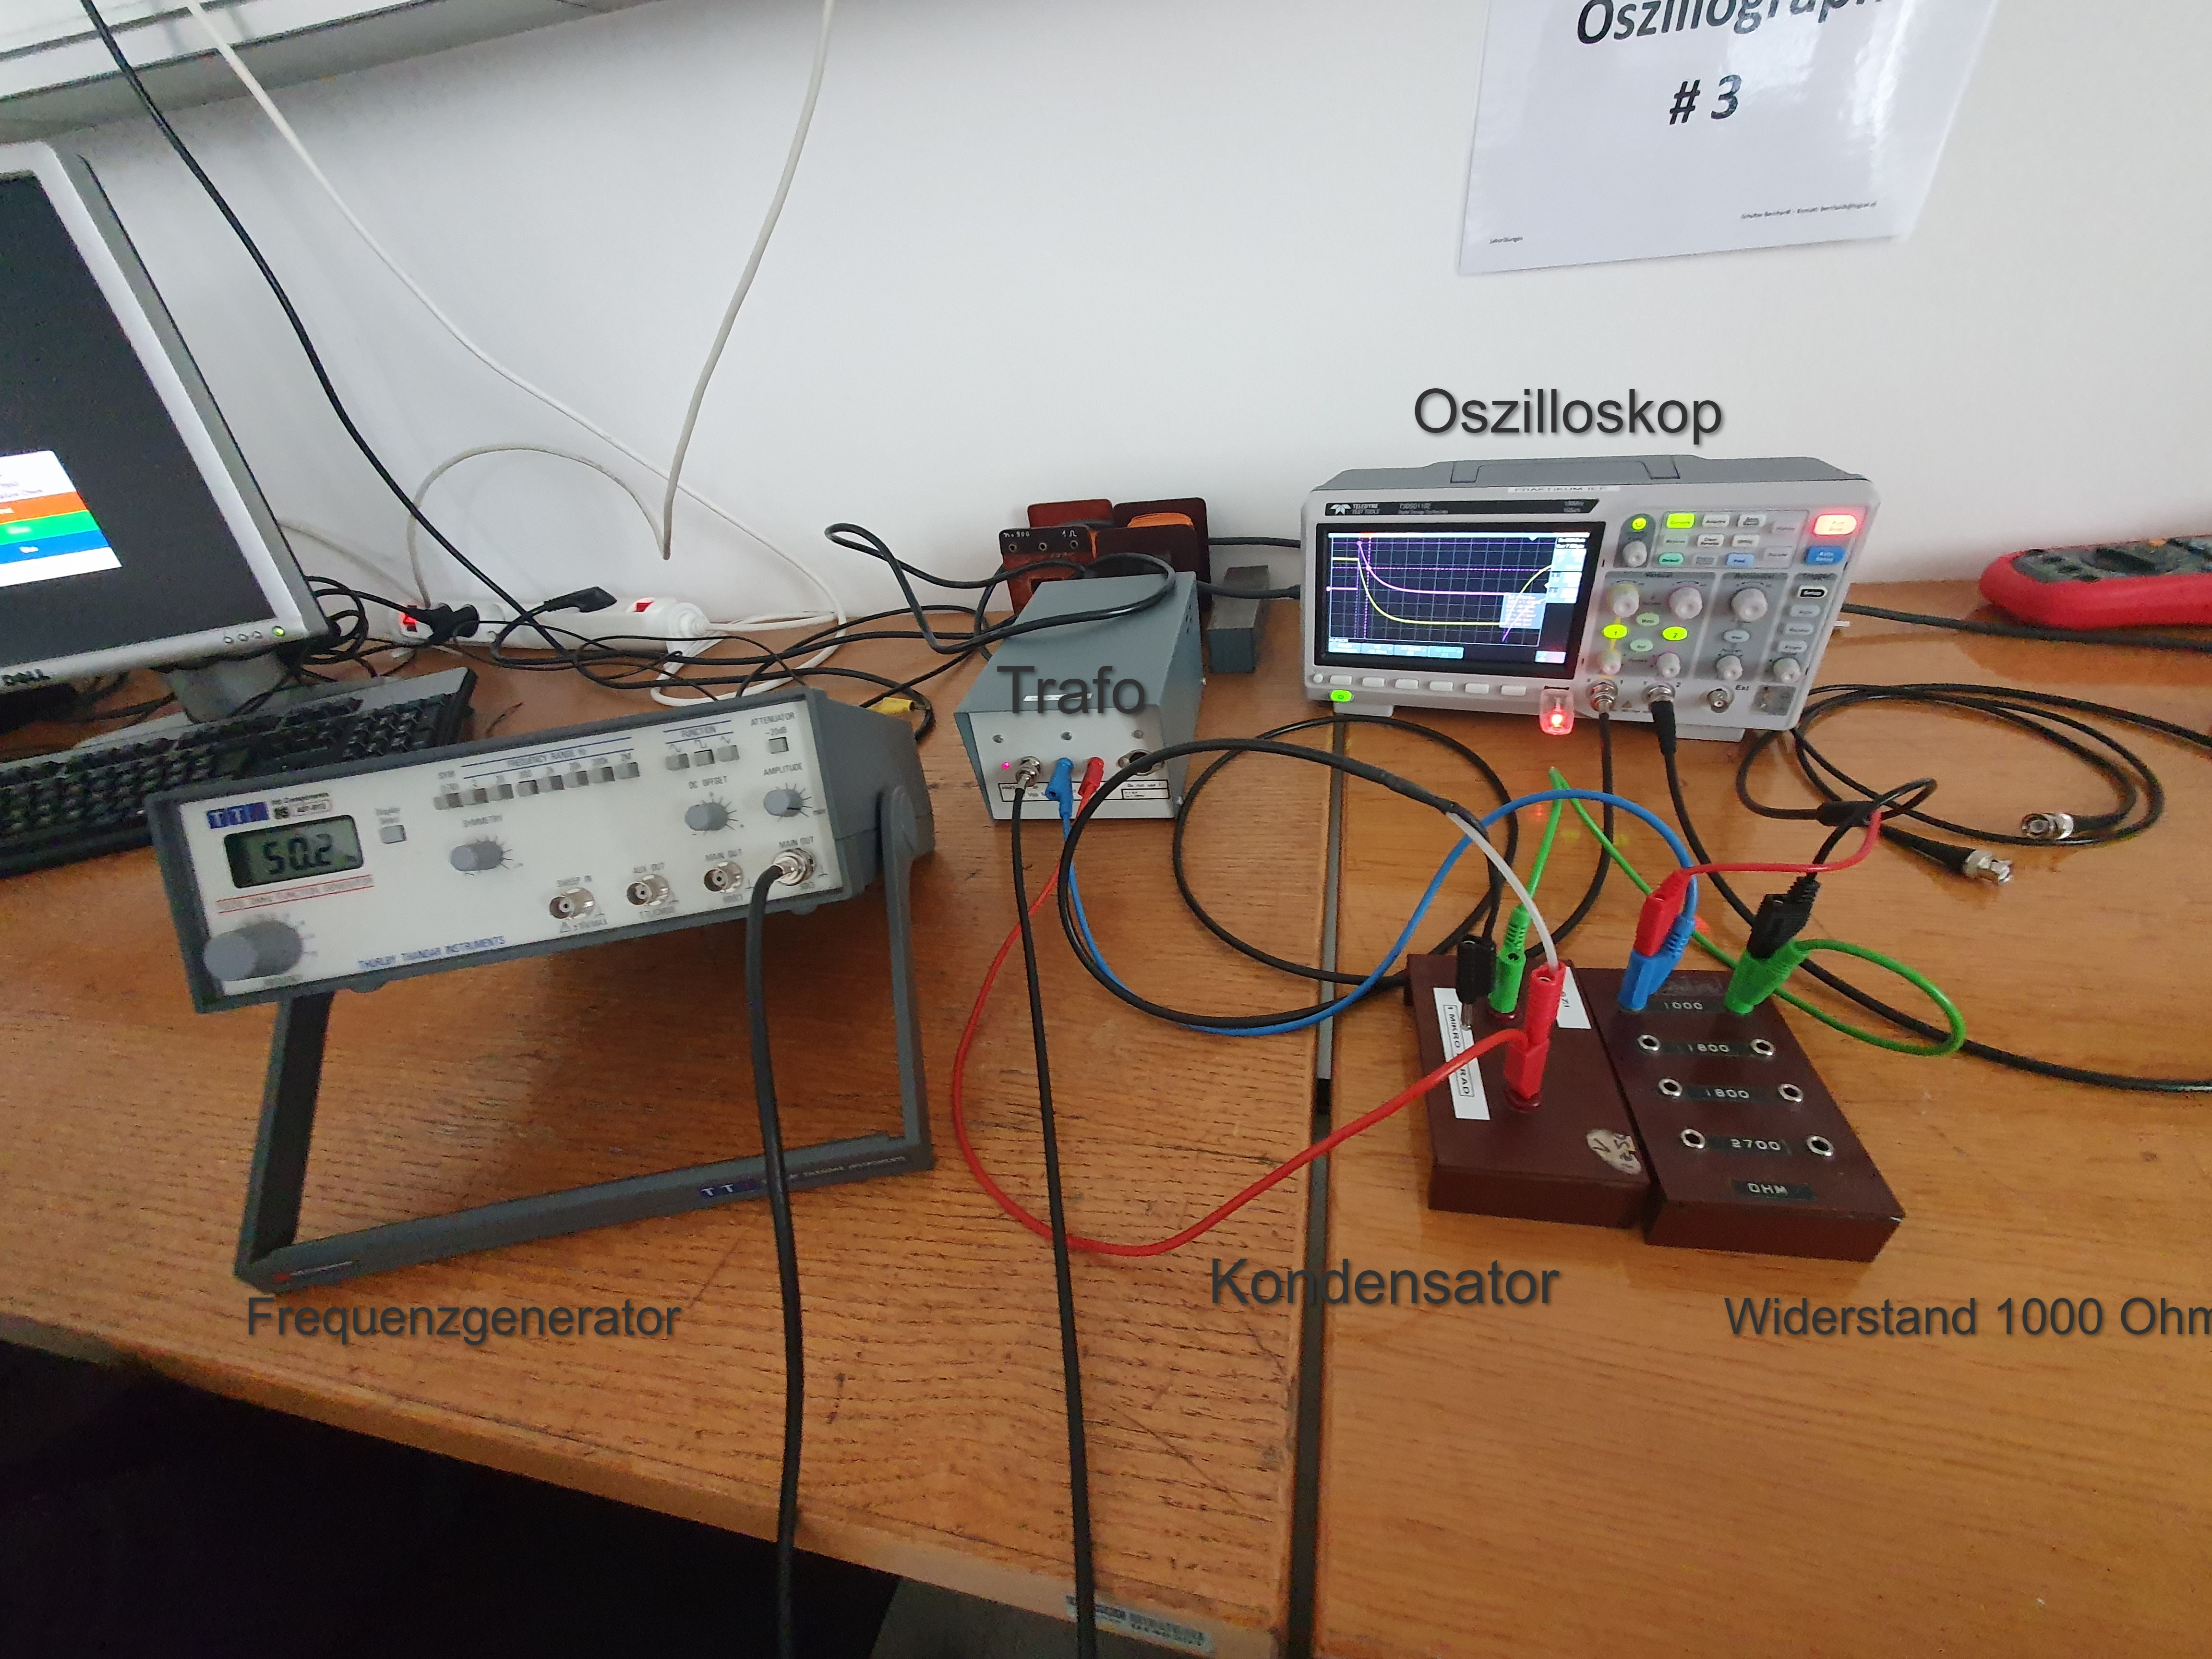
\includegraphics[width=0.6\linewidth, angle=0]{nudes/Aufbau Serienschaltung.jpg}
    \caption{Aufbau Serienschwingkreis}
    \label{fig:Aufbau Serienschwingkreis}
\end{figure} 

\noindent
Die dritte und letzte Schaltung ist im Gegensatz zu den anderen beiden sehr einfach strukturiert und setzt sich lediglich aus zwei Kompnenten zusammen:

\begin{figure}[H]
    \centering
    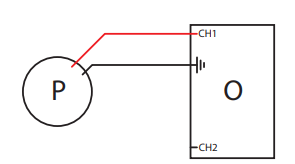
\includegraphics[width=0.6\linewidth, angle=0]{nudes/3.4 Eigenfrequenz.png}
    \caption{Aufbau Serienschaltung}
    \label{fig:Schaltplan Eigenfrequenzbestimmung}
\end{figure}

\noindent
Das Piezo P, welches im dritten Aufgabenteil an das Oszilloskop angeschlossen wird, ist in folgender Abbildung zu sehen:

\begin{figure}[H]
    \centering
    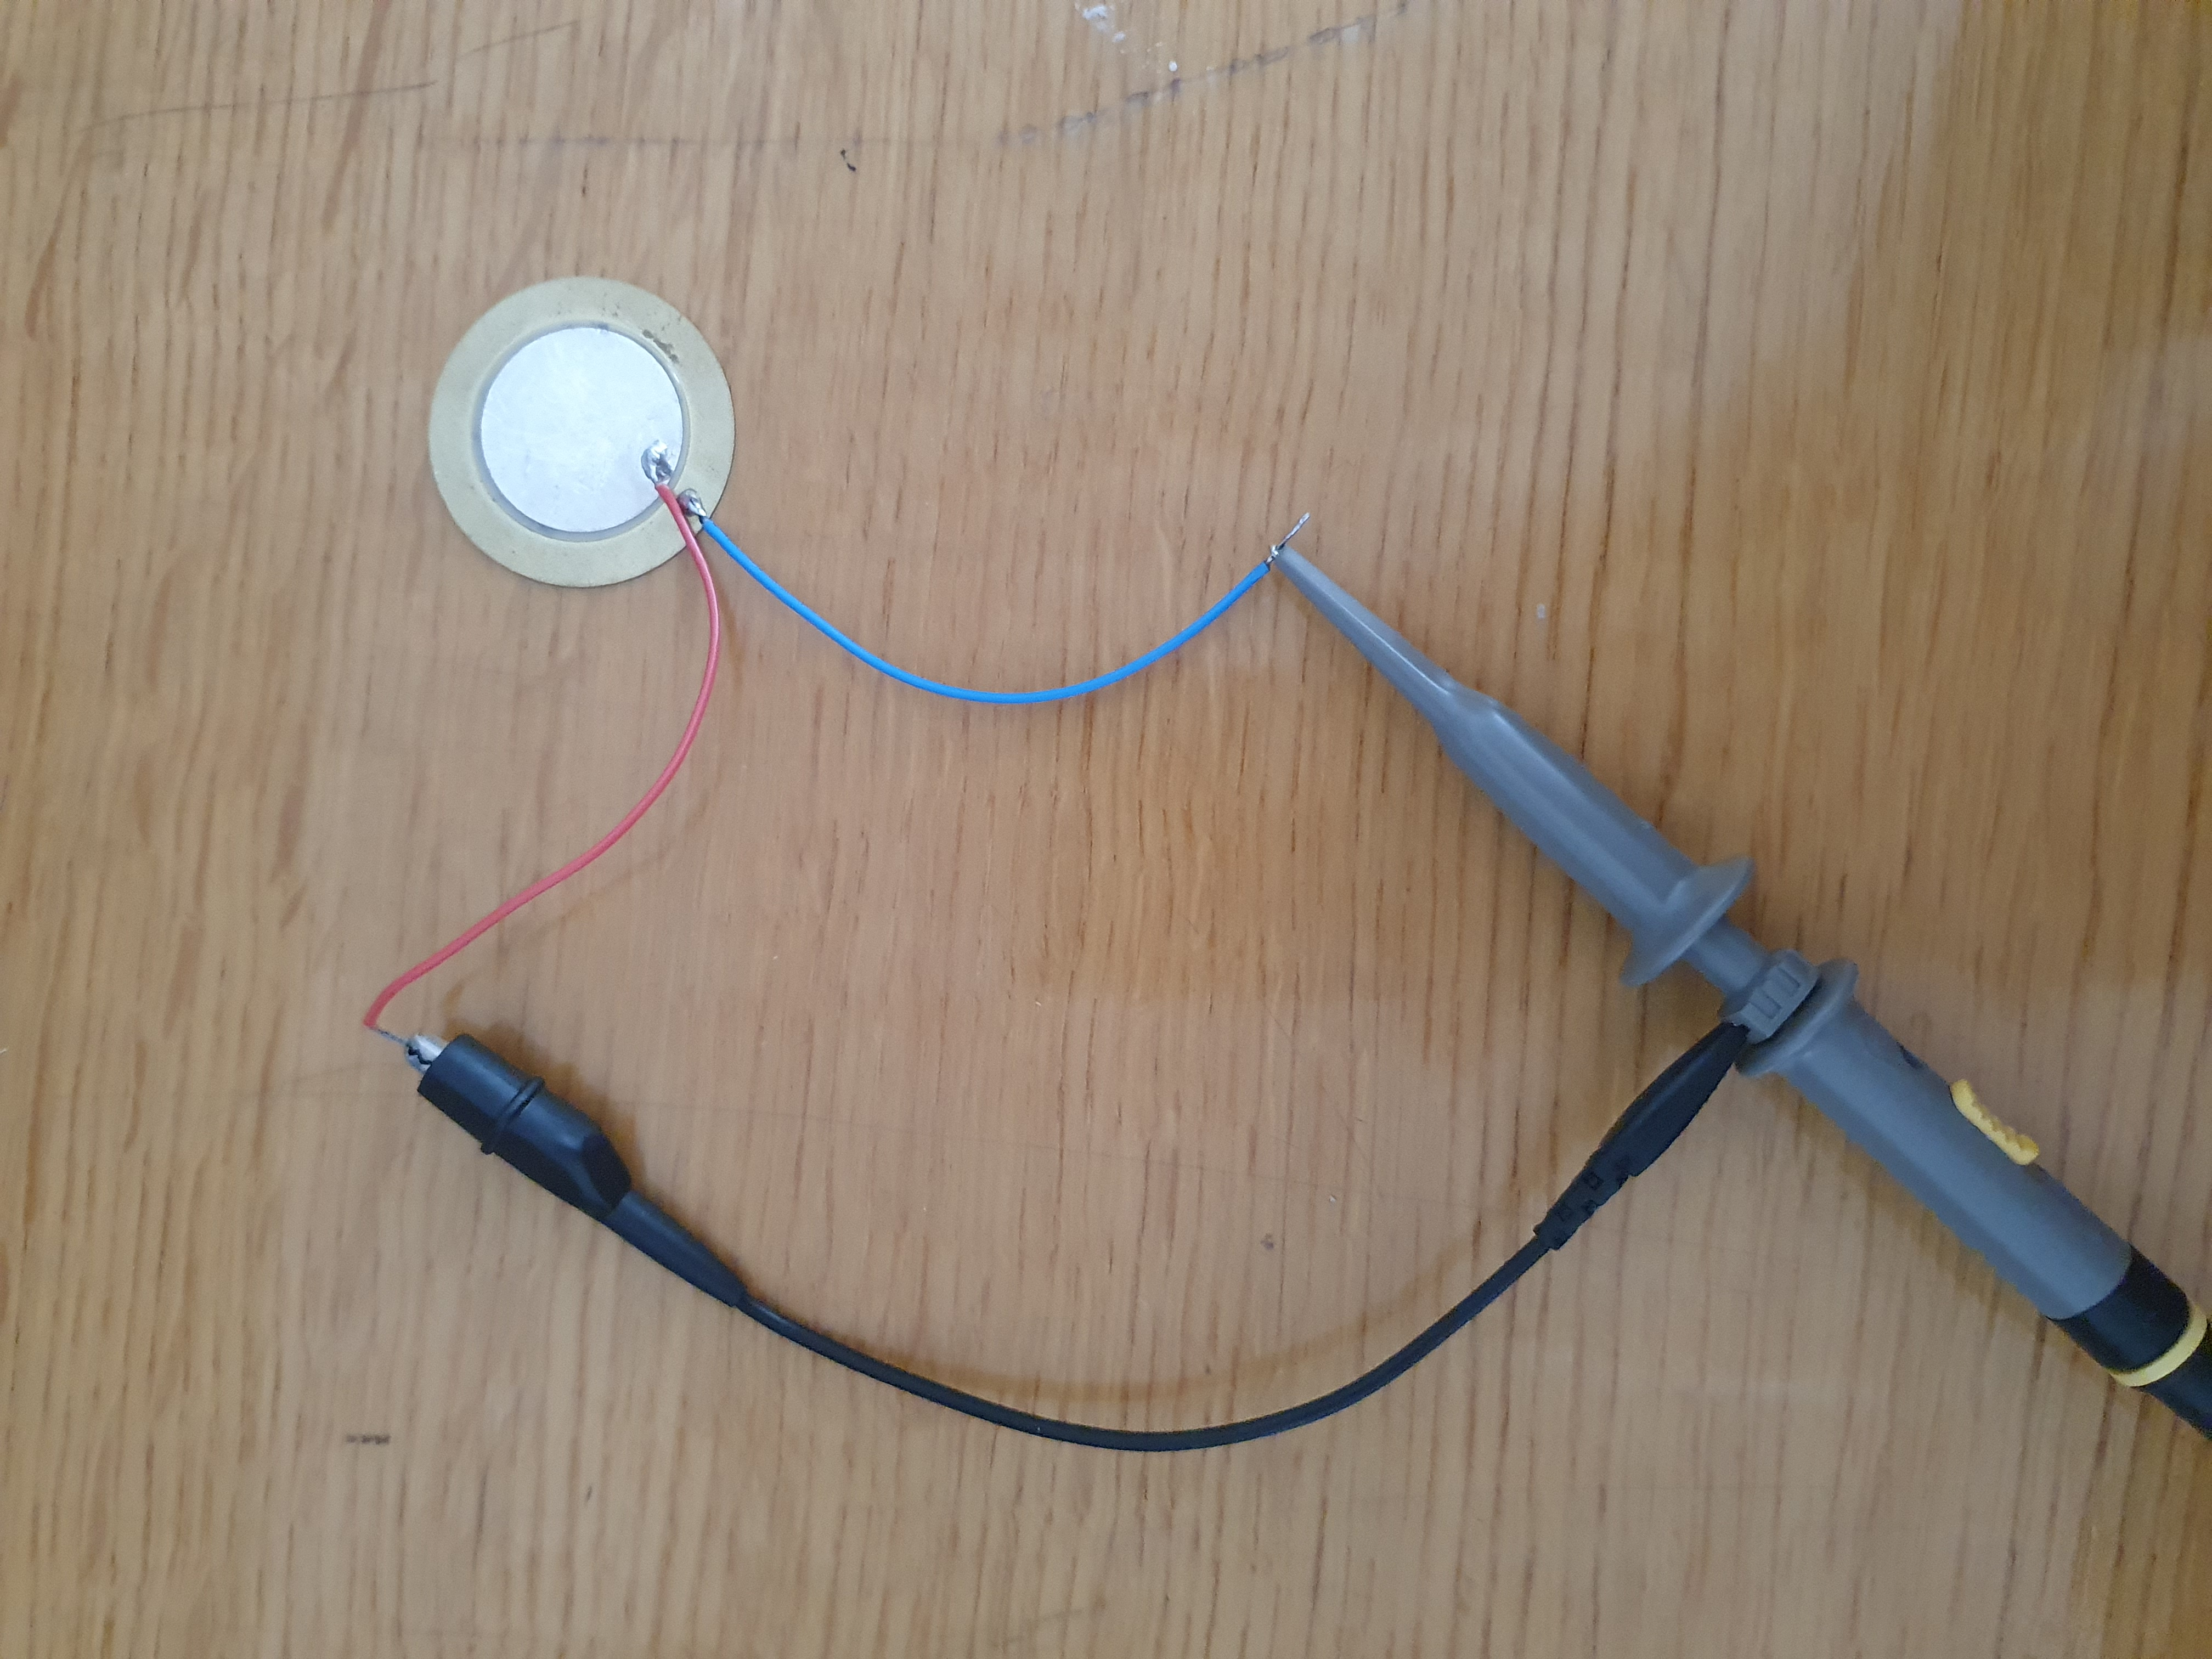
\includegraphics[width=0.6\linewidth, angle=0]{nudes/Piezo.jpg}
    \caption{Piezo}
    \label{fig:Piezo}
\end{figure}



\section{Geräteliste} %jo holt a listn ------------------------------

    \begin{table}[H]
        \centering
        \caption{Im Versuch verwendete Geräte und Utensilien.}
        \label{tab:geraete}
        \begin{tabular}{| l | l | l | l |}
            \hline
            Gerät   & Typ   & Gerätenummer  & Unsicherheit \\
            \hline
            Oszilloskop & {n.a} & {n.a} \\
            Trafo & {n.a} & {n.a} \\
            Frequenzgenerator & {n.a} & {n.a} \\
            Spule mit entfernbaren Eisenkern (n=500) & {n.a} & {n.a} \\
            50 Ohm Widerstand & {n.a} & {n.a} \\
            470 Ohm Potentiometer & {n.a} & {n.a} \\
            50 Ohm / 1000 Ohm Widerstand & {n.a} & {n.a} \\
            1 $\mu F$ Kondensator& {n.a} & {n.a} \\
            Piezo & {n.a} & {n.a} \\
            \hline
        \end{tabular}
    \end{table}


\section{Versuchsdurchführung \& Messergebnisse} %nachvollziehbar und klar dargestellt ------------------------------

Die Unsicherheiten

\subsection{Serienschaltung}

Zu Beginn des ersten Teiles des Versuchs wurde die Schaltung wie in Abbildung \ref{fig:Aufbau Serienschaltung} gezeigt aufgebaut. 
Am Frequenzgenerator wurde eine Frequenz von 50 Hz eingestellt und als sinusförmige Speisespannung an die Schaltung und in weiterer Folge an das Oszilloskop übermittelt werden. Damit soll nun der Spannungsverlauf als Funktion der Zeit grafisch dargestellt werden. \newline

\noindent
Weiters soll nun eine rechteckige Speisespannung mit erneut 50 Hz eingerichtet werden. Diesmal wird jedoch nicht die Phasenverschiebung ermittelt, sondern die Zerfallskonstante $\tau$.
Diese gibt jenen Zeitabschnitt an, in welchem die Spannung auf die Hälfte ihres Ursprungswertes (Halbwertszeit) gesunken ist. \newline

\noindent
Die Messergebnisse in Form von exportierten Bildern lassen sich in folgenden Abbildungen erkennen.

\begin{figure}[H]
    \centering
    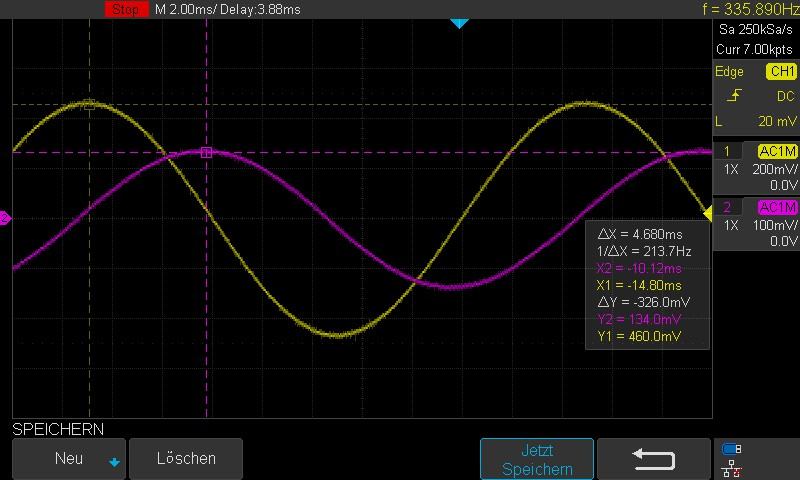
\includegraphics[width=0.6\linewidth, angle=0]{Messergebnisse/3.2/3.2a besser.jpg}
    \caption{Messergebnisse 3.2a}
    \label{fig:Messergebnisse3.2a}
\end{figure}

\begin{figure}[H]
    \centering
    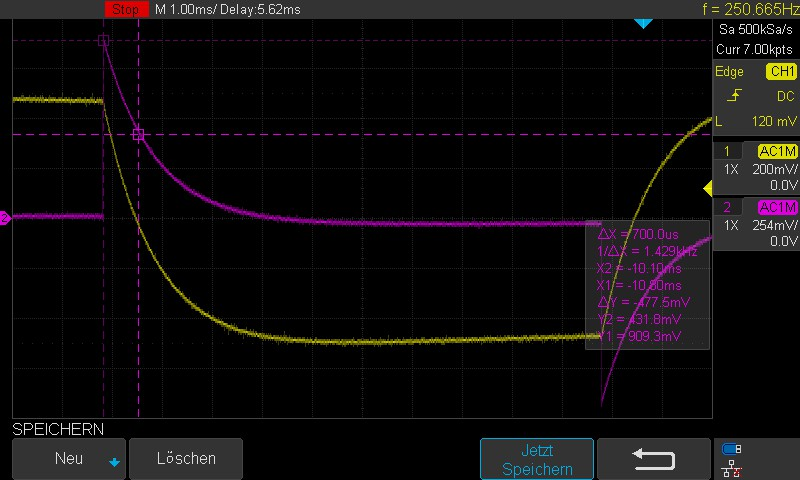
\includegraphics[width=0.6\linewidth, angle=0]{Messergebnisse/3.2/3.2b.jpg}
    \caption{Messergebnisse3.2b}
    \label{fig:Messergebnisse3.2b}
\end{figure}

\noindent 
Der Graph für den zweiten Teil des Versuches wurde außerdem als CSV Datei exportiert.


\subsection{Serienschwingkreis}

Im zweiten Teil des Experimentes soll nun die Serienschaltung zum in Abbildung \ref{fig:Schaltplan Serienschwingkreis} erwähnten Serienschwingkreis erweitert werden.
Mit dem neu hinzugefügten Potentiometer können nun durch einspeisen einer 50 Hz Rechtecksspannung die drei im Kapitel Grundlagen beschriebenen Fälle grafisch dargestellt werden. \newline

\noindent
Auch hier wurden wieder für jeden Fall ein Bild und ein CSV-File exportiert: \newline

\noindent
Der Kriechfall konnte bestimmt werden, indem das Potentiometer so adjustiert wurde, dass das Spannungsbild eine fallende Kurve bzw. den Kriechfall ergibt.

\begin{figure}[H]
    \centering
    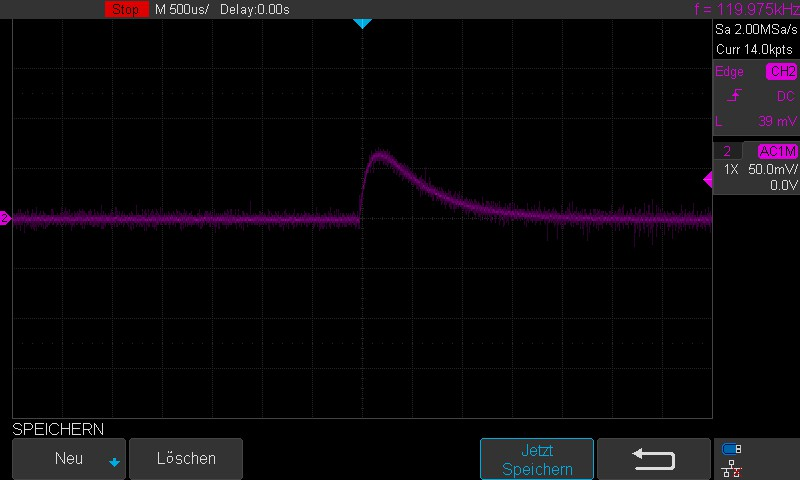
\includegraphics[width=0.6\linewidth, angle=0]{Messergebnisse/3.3 Kriechfall/KriechfallNahe.jpg}
    \caption{Messergebniss Kriechfall}
    \label{fig:MessergebnissKriechfall}
\end{figure}

\noindent
Für den Schwingfall wurde das Potentiometer ganz aufgedreht, bis die gedämpfte Schwingung am Oszilloskop zu sehen war.

\begin{figure}[H]
    \centering
    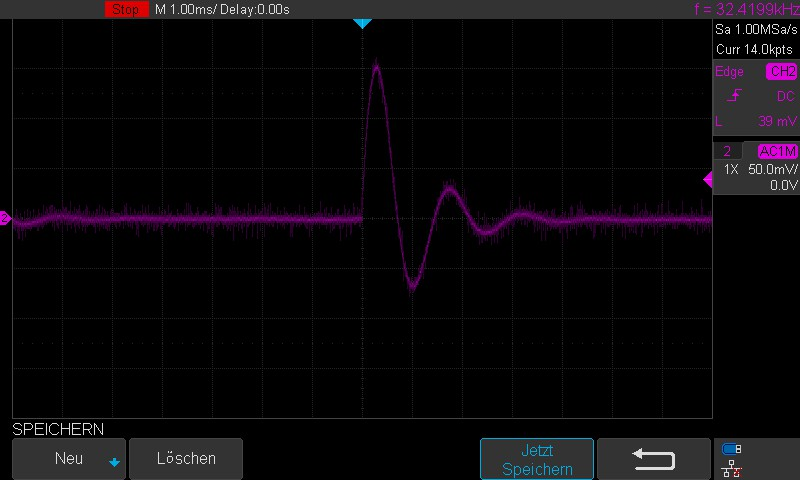
\includegraphics[width=0.6\linewidth, angle=0]{Messergebnisse/3.3 Schwingfall/SchwingfallNahe.jpg}
    \caption{Messergebniss Schwingfall}
    \label{fig:MessergebnissSchwingfall}
\end{figure}

\noindent
Um weiters den aperiodischen Grenzfall zu zeigen, musste das Potentiometer langsam zurückgedreht werden, bis der Übergang von Kriechfall zum Schwingfall erreicht wurde.
Dies lies sich daran erkennen, dass das untere Ende des Kriechfalles gerade zu "Schwingen" anfängt.

\begin{figure}[H]
    \centering
    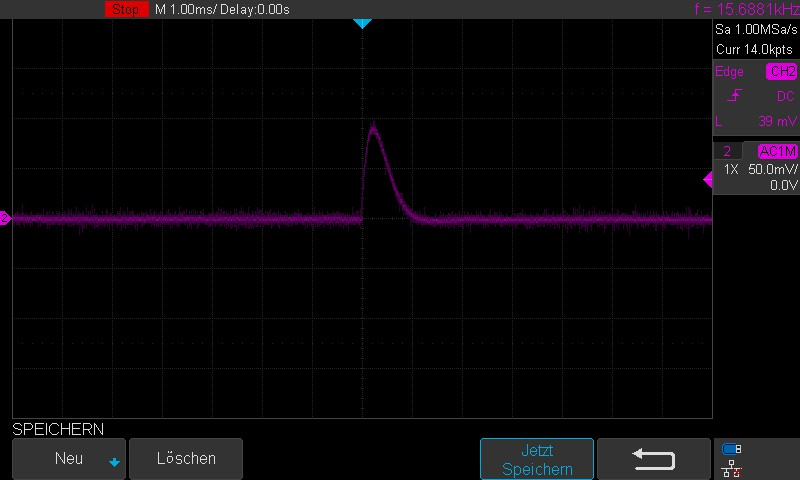
\includegraphics[width=0.6\linewidth, angle=0]{Messergebnisse/3.3 Grenzfall/GrenzfallNahe.jpg}
    \caption{Messergebniss aperiodischer Grenzfall}
    \label{fig:MessergebnissAperiodischerGrenzfall}
\end{figure}

\noindent
Außerdem sollte noch die Induktivität der Spule mit und ohne Eisenkern festgestellt werden. Hierfür soll der aperiodische Grenzfall jeweils einmal mit- und einmal ohne Eisenkern eingestellt werden. 
Dann wird mittels Potentiometer der Gesamtwiderstand beider Fälle gemessen und der Wert für die Auswertung festgehalten.

\begin{table}[H]
    \centering
    \caption{Messwerte Gesamtwiderstand}
    \label{tab:messwerteGesamtwiderstand}
    \begin{tabular}{| l | l |}
        \hline
        Gesamtwiderstand mit Eisenkern [Ohm] $\pm$ 1  & Gesamtwiderstand ohne Eisenkern [Ohm] $\pm$ 0.01 \\
        \hline
        298.0 & 115.8 \\
        \hline
    \end{tabular}
\end{table}


\subsection{Eigenfrequenz}

Im dritten und letzten Teil der Aufgabe soll die Eigenfrequenz eines Stuhles bestimmt werden. Dazu wurde die Schaltung aus den vorherigen Aufgaben durch das Piezo ersetzt.
Da das Piezo mittels Tastkopf mit dem Oszilloskop verbunden wurde, musste dessen Faktor (1x, 10x) beachtet und am Oszilloskop eingestellt werden. \newline

\noindent
Zur Bestimmung der Eigenfrequenz des Stuhles wurde das Piezo nun auf diesen gelegt und mit einem Metallzylinder beschwert. Dann konnte mit einem leichten Klopfen auf den Suhl die Schwingung am Oszilloskop beobachtet werden. 
Dabei wurden durch unterschiedliche Klopfstellen am Stuhl verschiedene Frequenzen beobachtet. Nach dem Klopfen auf die Stuhllehne wurde die Schwingung am Oszilloskop grafisch festgehalten.

\begin{figure}[H]
    \centering
    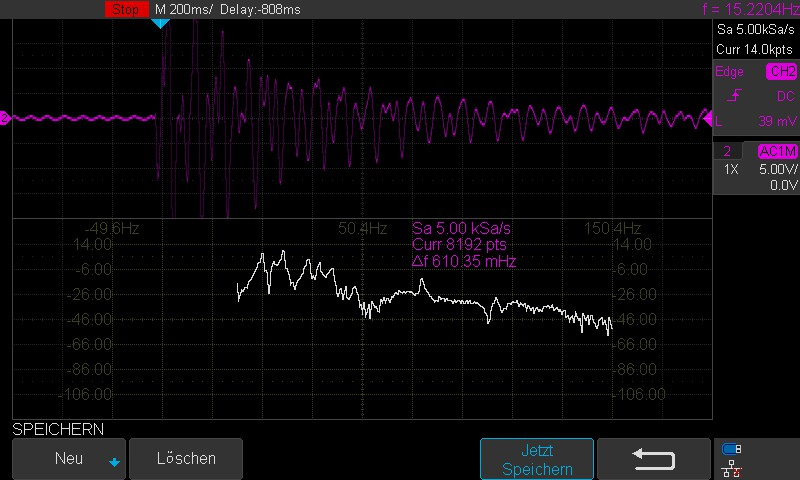
\includegraphics[width=0.6\linewidth, angle=0]{Messergebnisse/3.4EigenfrequenzStuhl/EigenfrequenzStuhl.jpg}
    \caption{Messergebniss Eigenfrequenz Stuhl}
    \label{fig:MessergebnissEigenfrequenzStuhl}
\end{figure}

\noindent
Letztenendes soll noch die Eigenfrequenz des Piezos selbst ermittelt werden. Hierzu wurde das Messgerät frei hängen gelassen und vorsichtig an der Messoberfläche (helle Seite) angetippt.
Die Ergebnisse konnten wiederum am Oszilloskop beobachtet werden, die Eigenfrequenz wurde diesesmal jedoch mit einer FastFourierTransformation (FFT) bestimmt.

\begin{figure}[H]
    \centering
    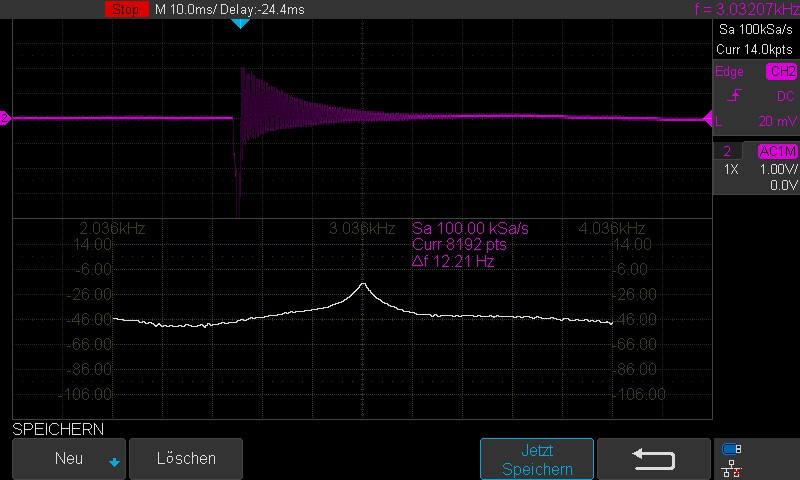
\includegraphics[width=0.6\linewidth, angle=0]{Messergebnisse/3.4 EigenfrequenzDing/DSO00001.jpg}
    \caption{Messergebniss Eigenfrequenz Piezo mit FFT}
    \label{fig:MessergebnissEigenfrequenzPiezo}
\end{figure}


\section{Auswertung und Unsicherheitsanalyse} %Nicht nur zahlen angeben ------------------------------

In der Auswertung werden zur erhöhten Genauigkeit durchgehend ungerundete Werte bis zu den Endergebnissen verwendet und nur zur Darstellung gerundet. \\
Zur Berechnung der Unsicherheiten wird, wenn nicht anders angegeben, die Größtunsicherheitsmethode verwendet.

\subsection{Serienschaltung}

Wie in Abbildung \ref{fig:Messergebnisse3.2a} erkennbar ist, beträgt der mittels Oszilloskoptools gemessene Zeitunterschied $\Delta t$ 4.7 ms. Setzt man dies nun gemeinsam mit der verwendeten Frequenz von 50 Hz in Formel \ref{eq:Phasenversatz} ein, so erhält man für den Phasenversatz einen Wert von $\Phi$ = 84.6°.



\subsection{Serienschwingkreis}

\subsection{Eigenfrequenz}



\section{Diskussion} %diskussion der Unsicherheiten und Ergebnisse und evtl. verlgeich mit Literatur ------------------------------


\section{Zusammenfassung} %klare, übersichtliche vollständige beantwortung der Aufgabenstellung ------------------------------


\printbibliography[heading=bibintoc]
\end{document}
